% Journal version for Annals of Operations Research (Springer Nature).
% Bootstrapped from ../opt2026.tex by tools/from_opt.py; hand-edited after.
%
% Uses the Springer Nature class sn-jnl.cls when it is present in this
% directory (download the "Journal article template package" from
% https://www.springernature.com/gp/authors/campaigns/latex-author-support
% and copy sn-jnl.cls and the sn-*.bst files here); otherwise falls back to
% article so that the draft builds while the content is being written.
\IfFileExists{sn-jnl.cls}{%
  \documentclass[pdflatex,sn-apa]{sn-jnl}%  AOR: APA 7 references
  \newif\ifsnjnl\snjnltrue
}{%
  \documentclass[11pt,a4paper]{article}
  \newif\ifsnjnl\snjnlfalse
  \usepackage[margin=2.5cm]{geometry}
  \usepackage{amsmath,amssymb,amsfonts,amsthm}
  \usepackage[authoryear,round]{natbib}
  \usepackage{graphicx}
  \usepackage{hyperref}
  \newtheorem{theorem}{Theorem}
  \newtheorem{lemma}[theorem]{Lemma}
  \newtheorem{proposition}[theorem]{Proposition}
  \newtheorem{corollary}[theorem]{Corollary}
  \newtheorem{remark}[theorem]{Remark}
  \newtheorem{assumption}[theorem]{Assumption}
}
\ifsnjnl
  % the Springer class does not load the AMS packages itself; the
  % template's preamble loads these before its theorem definitions
  \usepackage{amsmath,amssymb,amsfonts,amsthm}
  \usepackage{manyfoot}
  \theoremstyle{thmstyleone}
  \newtheorem{theorem}{Theorem}
  \newtheorem{lemma}[theorem]{Lemma}
  \newtheorem{proposition}[theorem]{Proposition}
  \newtheorem{corollary}[theorem]{Corollary}
  \theoremstyle{thmstyletwo}
  \newtheorem{remark}[theorem]{Remark}
  \newtheorem{assumption}[theorem]{Assumption}
\fi
\usepackage[utf8]{inputenc}
\usepackage[T1]{fontenc}
\usepackage{mathtools}
\usepackage{booktabs}
\usepackage{array}
\usepackage[expansion=false]{microtype}
\usepackage{xcolor}
\usepackage[ruled,linesnumbered]{algorithm2e}
\usepackage[section]{placeins}
% the OPT class wrapped algorithm2e's float as "algorithm2e"; keep the name
\newenvironment{algorithm2e}[1][t]{\begin{algorithm}[#1]}{\end{algorithm}}
\hypersetup{hidelinks}
\graphicspath{{../}{../figs/}}
\setlength{\emergencystretch}{2em}
\newcommand{\todo}[1]{\textcolor{red}{[TODO: #1]}}

\newcommand{\conv}{\operatorname{conv}}
\newcommand{\PW}{\mathrm{PW}}
\newcommand{\ip}[2]{\langle #1, #2 \rangle}
\newcommand{\norm}[1]{\lVert #1 \rVert}
\newcommand{\R}{\mathbb{R}}
\newcommand{\gFW}{g^{\mathrm{FW}}}
\newcommand{\gA}{g^{\mathrm{A}}}
\newcommand{\gPW}{g^{\mathrm{PW}}}
\newcommand{\UB}{\mathrm{UB}}
\newcommand{\LB}{\mathrm{LB}}


\begin{document}

\ifsnjnl
\title[Guarded block transfers for polytope distance]{Guarded block transfers for polytope distance: linear convergence, gap-certified screening, and when aggregation pays}
\author*[1]{\fnm{Mayank} \sur{Gupta}}\email{iammayankg@gmail.com}
\affil*[1]{\orgname{\todo{affiliation}}, \orgaddress{\city{\todo{city}}, \country{\todo{country}}}}
\abstract{Training a hard-margin support vector machine is the distance problem
between two convex hulls, which the Triangle Algorithm solves with a
certified duality gap. We study \emph{guarded block transfers}: $k$
Mitchell--Demyanov--Malozemov transfers per scan are aggregated into
one exact line search, guarded by a comparison with the single best
transfer, and replaced by an away step when the leading transfer is
capacity-clipped. On the Minkowski-difference polytope we prove linear
convergence, with constants explicit in the pyramidal width and no
combinatorial swap-step bounds, and a finite activation bound for
gap-safe screening. We then ask when
aggregation pays. The gain of a block over the single transfer has an
exact expression in two quantities the guard
already computes, the summed relative pair gain and the loss to
combining the directions; under strict complementarity and
non-degeneracy every drop step occurs before an explicit
identification iteration; and a fitted work model gives the block size
that minimises the per-iteration term, which the solver sets
adaptively from the measured combination loss. On five LIBSVM problems aggregation pays only
where per-iteration work rather than column computation dominates, by
at most 2.8 times. On the one separable real dataset the solver ties
LIBSVM; on kernel $L_2$ margins it beats our own implementations of
blended pairwise conditional gradients and, where kernel columns are
expensive, of sequential minimal optimisation, but not LIBSVM with the
kernel in memory; on dense-support $L_2$ margins it is at least two
orders of magnitude slower than LIBLINEAR.}
\keywords{polytope distance, Frank--Wolfe methods, Triangle Algorithm, support vector machines, safe screening, linear convergence}
\maketitle
\else
\title{Guarded block transfers for polytope distance: linear convergence, gap-certified screening, and when aggregation pays}
\author{Mayank Gupta\thanks{\todo{affiliation}; \texttt{iammayankg@gmail.com}}}
\date{}
\maketitle
\begin{abstract}
Training a hard-margin support vector machine is the distance problem
between two convex hulls, which the Triangle Algorithm solves with a
certified duality gap. We study \emph{guarded block transfers}: $k$
Mitchell--Demyanov--Malozemov transfers per scan are aggregated into
one exact line search, guarded by a comparison with the single best
transfer, and replaced by an away step when the leading transfer is
capacity-clipped. On the Minkowski-difference polytope we prove linear
convergence, with constants explicit in the pyramidal width and no
combinatorial swap-step bounds, and a finite activation bound for
gap-safe screening. We then ask when
aggregation pays. The gain of a block over the single transfer has an
exact expression in two quantities the guard
already computes, the summed relative pair gain and the loss to
combining the directions; under strict complementarity and
non-degeneracy every drop step occurs before an explicit
identification iteration; and a fitted work model gives the block size
that minimises the per-iteration term, which the solver sets
adaptively from the measured combination loss. On five LIBSVM problems aggregation pays only
where per-iteration work rather than column computation dominates, by
at most 2.8 times. On the one separable real dataset the solver ties
LIBSVM; on kernel $L_2$ margins it beats our own implementations of
blended pairwise conditional gradients and, where kernel columns are
expensive, of sequential minimal optimisation, but not LIBSVM with the
kernel in memory; on dense-support $L_2$ margins it is at least two
orders of magnitude slower than LIBLINEAR.
\end{abstract}
\noindent\textbf{Keywords:} polytope distance; Frank--Wolfe methods; Triangle Algorithm; support vector machines; safe screening; linear convergence
\fi

\section{Introduction}

Given two finite point sets $V,W\subset\R^d$, the \emph{polytope
distance problem} asks for the closest pair of points of their convex
hulls, equivalently for the minimum-norm point of the Minkowski
difference $\conv(V)-\conv(W)$. It is one of the oldest problems of
computational convexity: Gilbert's procedure \citep{gilbert1966}, the
Mitchell--Demyanov--Malozemov (MDM) algorithm \citep{mdm1974} and
Wolfe's minimum-norm-point method \citep{wolfe1976} all solve it by
moving weight between vertices, and all are instances of the
conditional-gradient scheme of \citet{frankwolfe1956}. Kalantari's
Triangle Algorithm (TA) began with the convex-hull membership problem
and its \emph{distance duality} \citep{kalantari2015}, published in
this journal; \citet{kalantari2019} carried it to two hulls, where
TA~I decides whether the hulls intersect and TA~II returns the
distance with a certified interval $[\LB,\UB]$ from a pair of parallel
supporting hyperplanes, the support-function bound of
\citet{gilbert1966} and Wolfe's stopping test in the two-hull setting.
The problem's best-known
application is the hard-margin support vector machine (SVM): the
optimal separator is the perpendicular bisector of the closest pair and
the margin is half the hull distance \citep{bennett2000duality,
keerthi2000}, and the $L_2$ soft margin, the $\nu$-SVM and the kernel
variants are the same problem on augmented, reduced or feature-space
hulls (Section~\ref{app:red}).

This paper keeps two parts of the Triangle Algorithm and replaces the
third. It keeps the distance duality and the certificate: every lower
bound below comes from the parallel supporting hyperplanes of
\citet{kalantari2019}, and the stopping rule is the certified relative
gap. It keeps TA~I as the intersection test. It replaces the pivot
step, a move toward a single vertex, by the MDM weight transfer from
the worst active vertex to the best candidate, which is the pairwise
Frank--Wolfe (FW) step of \citet{lj2015} on the difference polytope,
and asks how much of the $O(n)$ scan that selects the transfer can be
reused across several transfers without weakening the guarantee. The
answer is a \emph{guarded block transfer}: $k$ transfers per scan are
aggregated into one exact line search, guarded by an $O(k^2)$
comparison with the single best transfer, and replaced by an away step
when the leading transfer is capped. In the terms of the
FW literature the method is pairwise FW with the TA certificate, a
block step rule and an away fallback; we keep the name enhanced TA
(ETA), after \citet{gupta2026}, whose dot-product caching it also
retains.

\paragraph{Contributions.}
\begin{enumerate}\setlength\itemsep{0pt}
\item \textbf{Guarded block transfers} (Section~\ref{sec:alg}): pair the top-$k$
receivers with the worst-$k$ active donors, take one exact line search
along the aggregated direction, \emph{guard} it by an $O(k^2)$
comparison with the single MDM step, and fall back to an away step on
capped iterations.
\item \textbf{Linear convergence with constants explicit in the
pyramidal width} (Theorem~\ref{thm:linear}, Corollary~\ref{cor:std}): on
$Z=\conv(V)-\conv(W)$ the guarded block algorithm inherits the
pyramidal-width rate of pairwise FW \citep{lj2015} up to a factor
four, and the away fallback replaces the combinatorial swap-step bound
by drop-step counting with up to $k$ added indices per step (cf.\
\citealp{tsuji2022}).
\item \textbf{Screening activation with explicit constants}
(Theorem~\ref{thm:activation}): the TA certificate is the FW gap divided
by the distance (Lemma~\ref{lem:gapid}), so gap-safe screening
\citep{ndiaye2017} applies, and we bound the iteration by which it has
removed every zero-weight point off the optimal faces.
\item \textbf{A regime study on real data} (Section~\ref{sec:exp}): two
batteries on five LIBSVM datasets locate the boundary between the
sparse-support regime, where the certified solver competes with LIBSVM,
and the dense-support regime, where it does not.
\item \textbf{When aggregation pays} (Sections~\ref{sec:pay}
and~\ref{sec:pay-meas}): (a) the exact gain ratio of a block over the
single MDM step at the same iterate, $Q(2-\chi)$ or $Q/\chi$ in two
observable numbers, $Q$ the summed pair gains relative to the leading
pair and $\chi$ the ratio of the combined direction's squared norm to
its directional derivative (Proposition~\ref{prop:ratio}); (b) an
identification theorem: under strict complementarity and
non-degeneracy all drop steps occur before an explicit iteration and
none afterwards (Theorem~\ref{thm:ident}); (c) a conditional iteration
bound (Corollary~\ref{cor:work}) and a timing model with the block size
that minimises it; (d) isolated per-step measurements of every quantity
in the model on five real cells; (e) an adaptive block size driven by
the measured $\chi$, checked on cells not used to set its constants.
\end{enumerate}
Code, proofs, numerical checks and experiment scripts are in the public
repository (\todo{URL}).

\section{Related work}\label{sec:related}

\paragraph{Polytope distance in operations research.}
\citet{gilbert1966}, \citet{mdm1974} and \citet{wolfe1976} give the
classical minimum-norm-point methods; \citet{lopez2015}
analyse MDM's convergence, and \citet{kalantari2015,kalantari2019}
develop the Triangle Algorithm and its separating-hyperplane theorem
for the convex-hull membership and distance problems. \citet{pena2016}
relate von Neumann's algorithm and FW with away steps on the same
polytope feasibility problem and obtain linear rates through a
condition number of the polytope, the closest relative of the constants
in Theorem~\ref{thm:linear}.

\paragraph{Frank--Wolfe variants.} The conditional-gradient method of
\citet{frankwolfe1956}, revisited by \citet{jaggi2013}, converges
sublinearly on polytopes; away steps restore a linear rate under
strong convexity with an interior-optimum condition \citep{guelat1986}
and, for general polytopes, with the pyramidal width \citep{lj2015};
\citet{garber2016} obtain linear rates through a local linear oracle
instead, \citet{beck2017} extend the away-step rate to non-strongly
convex composite objectives, \citet{pena2019} give the facial distance
as a computable alternative to the pyramidal width, and
\citet{braun2022} survey the field. Pairwise FW, the MDM transfer, carries a combinatorial
swap-step bound that blended pairwise conditional gradients (BPCG)
\citep{tsuji2022} and the short-step chains of \citet{rinaldi2023}
remove; boosted FW \citep{combettes2020} aggregates several atoms into
one direction by gradient alignment, and block-coordinate FW
\citep{lacoste2013bcfw} blocks over coordinates of a product domain.
Our step differs from each of these in one respect, made precise
below.

\paragraph{SVM training as polytope distance.} The nearest-point view
of the SVM is due to \citet{keerthi2000} and \citet{bennett2000duality},
whose reduced convex hulls, the soft convex hulls of \citet{crisp2000}
and the geometric formulation of \citet{mavroforakis2006} give the
$\nu$-SVM, with the iterative maximal-margin algorithm of
\citet{franc2003}; core-set and FW solvers for the same problem are
\citet{tsang2005,gartner2009,clarkson2010,nanculef2014}. The
production solvers we compare against are sequential minimal
optimisation (SMO) \citep{platt1998} as implemented in LIBSVM
\citep{chang2011} and the primal trust-region Newton solver of
LIBLINEAR \citep{fan2008}, both through scikit-learn
\citep{pedregosa2011}, and our own SMO.

\paragraph{Screening and identification.} Gap-safe rules
\citep{fercoq2015,ndiaye2017,shibagaki2016} screen with a radius from
the duality gap and identify the equicorrelation set, a superset of the
support, in finite time; the active-set complexity of away-step FW
\citep{bomze2020} and the strict-complementarity bounds of
\citet{garber2020} give identification from the algorithm's side.
\citet{ogawa2013} adapted the feature-elimination rules of
\citet{elghaoui2012} to the screening of non-support vectors, and
\citet{wang2014} reduce the data exactly. The rule of
Section~\ref{sec:alg} is the gap-safe sphere of \citet{ndiaye2017}
with the TA certificate as its dual pair; what is new in
Theorem~\ref{thm:activation} is the activation bound, and
Theorem~\ref{thm:ident} is the corresponding identification statement.

\paragraph{What is different here.} Boosted FW builds its direction by
greedily aligning a combination of atoms with the negative gradient, at
several oracle calls per iteration, and inherits the FW rate through an
alignment condition; our block fixes the pair coefficients $\gamma_j$
from one scan and relies on the guard, not on alignment, for its rate.
BPCG removes pairwise FW's swap-step bound with a guard between the
pairwise step and a FW step; our guard compares an aggregated block of
$k$ transfers with the single MDM step and falls back to an away step,
so the drop-step count of away-step FW carries over with up to $k$
(two-sided: $2k$) indices added per non-drop step, and each non-drop
case-(b) step is at least as good as the best of the block, MDM, away
and toward candidates. BPCG's linear rate has the same pyramidal-width
form as Theorem~\ref{thm:linear}; it is compared on the same real cells
in Table~\ref{tab:bpcg}. Block-coordinate FW and the short-step chains
of \citet{rinaldi2023} act on the domain decomposition and on the step
length, not on the direction. Wolfe's method minimises over the affine
hull of a corral at every iteration, which does not fit the
one-column-per-iteration oracle model of the comparison, and was not
run. A bound on the pyramidal width of the difference atom set
$A=\{v_i-w_j\}$ in terms of the two class hulls is open, and none can
be dimension-free: $V=\{0,e_1\}$ and $W=\{0,-(e_1+\epsilon e_2)\}$,
translated apart, have well-conditioned class hulls while the four
difference atoms span a parallelogram of height $\epsilon$, so that
$\PW(A)\le\epsilon$.

\section{Setting}\label{sec:setting}

Let $V=\{v_1,\dots,v_n\}$, $W=\{w_1,\dots,w_m\}\subset\R^d$. The
polytope distance problem is
\begin{equation}\label{eq:P}
  \min_{p\in\conv(V),\ q\in\conv(W)} \ \tfrac12\norm{p-q}^2 .
\end{equation}
Writing $z=p-q$ and $Z:=\conv(V)-\conv(W)=\conv\{v_i-w_j\}$,
\eqref{eq:P} is the minimum-norm-point problem $\min_{z\in Z}F(z)$,
$F(z)=\tfrac12\norm z^2$, whose objective is $1$-strongly convex and
$1$-smooth. Let $z^*$ be the minimiser, $\delta^*=\norm{z^*}$,
$h(z)=F(z)-F(z^*)$, $M=\operatorname{diam}(Z)$ and
$\delta=\PW(A)>0$ the pyramidal width \citep{lj2015} of the atom set
$A=\{v_i-w_j\}$ (a property of the atom set, not of $Z$ alone).

The algorithm keeps simplex weights $\alpha$ on $V$, $\beta$ on $W$
(iterate $z_t$ after $t$ iterations),
with $p=\sum\alpha_iv_i$, $q=\sum\beta_jw_j$; the induced product
representation $\lambda_{ij}=\alpha_i\beta_j$ of $z$ over the atoms
$v_i-w_j$ has support $\operatorname{supp}\alpha\times\operatorname{supp}\beta$.
With $g=-\nabla F(z)=q-p$, the \emph{side scores} are
$s^V_i=\ip{g}{v_i}$ and $s^W_j=\ip{p-q}{w_j}$, maintained incrementally
from cached arrays.

\paragraph{Certificate.} For any iterate, $\UB=\norm z$ and
$\LB=\min_{u\in Z}\ip{z}{u}/\norm z=\big(\min_i\ip{z}{v_i}-\max_j\ip{z}{w_j}\big)/\UB$
satisfy $\LB\le\delta^*\le\UB$; the TA stops when the certified
relative gap $(\UB-\LB)/\UB$ is at most $\varepsilon$. The $L_2$ soft margin with regularisation
parameter $C$, the $\nu$-SVM and the kernel variants reduce to
\eqref{eq:P} exactly (augmented coordinates that turn the Gram matrix
$K$ into $K+I/C$; reduced convex hulls; feature-space images), see
Section~\ref{app:red}.

\paragraph{Gaps.} $\gFW=\max_{u\in Z}\ip{g}{u}-\ip{g}{z}$,
$\gA=\ip{g}{z}-\min_{u\in\operatorname{supp}\lambda}\ip{g}{u}$,
$\gPW=\gFW+\gA$. Because $\ip{g}{v_i-w_j}=s^V_i+s^W_j$ is separable and
the support is a product set, each gap splits into a $V$-side and a
$W$-side term computable from the score arrays in $O(n+m)$
(Lemma~\ref{lem:sep}), written $\gPW_V,\gPW_W$ (likewise for FW and A),
with $\gPW_{\text{side}}$ the term of the side being stepped; a transfer
$v_r-v_u$ on the $V$ side is a pairwise direction of $Z$
(Lemma~\ref{lem:side}).

\begin{lemma}[Separability]\label{lem:sep}
With the product representation, $\gPW=\gPW_V+\gPW_W$ where
$\gPW_V=\max_is^V_i-\min_{i\in\operatorname{supp}\alpha}s^V_i\ge0$ and
$\gPW_W$ likewise; the same holds for $\gFW$ and $\gA$.
\end{lemma}
\begin{proof}
$\ip{g}{v_i-w_j}=s^V_i+s^W_j$ is separable and the support is a product
set, so the max over atoms and the min over the support separate. Each
side term is nonnegative: the FW term is the maximum score minus the
weighted mean of the support scores, the away term is that mean minus
the support minimum, and a weighted mean lies between the minimum and
the maximum.
\end{proof}

\begin{lemma}[Side transfers are $Z$-pairwise directions]\label{lem:side}
For $\alpha_u>0$ and any $b\in\operatorname{supp}\beta$,
$v_r-v_u=(v_r-w_b)-(v_u-w_b)$ is a difference of an atom of $Z$ and an
atom in the support, and the transfer with $0\le\gamma\le\alpha_u$ realises
$z\leftarrow z+\gamma(v_r-v_u)$ inside $Z$. The side capacity
$\alpha_u=\sum_{b}\alpha_u\beta_b$ is the total weight of the product
atoms $v_u-w_b$, $b\in\operatorname{supp}\beta$: the side transfer is
the sum of the atom-pair transfers of masses $\gamma\beta_b$ from
$v_u-w_b$ to $v_r-w_b$, and for $r\ne u$ this weight update is feasible
exactly when $0\le\gamma\le\alpha_u$; hence every such transfer remains
in $Z$.
\end{lemma}

\begin{table}[t]\centering\scriptsize\setlength{\tabcolsep}{3pt}
\caption{Notation. Symbols with a second, conventional meaning in one
place only are listed with both.}\label{tab:notation}
\begin{tabular}{@{}l>{\raggedright\arraybackslash}p{4.8cm}l>{\raggedright\arraybackslash}p{5.2cm}@{}}\toprule
$V,W$; $n,m$; $d$ & point sets, their sizes, dimension & $Z$, $A$ & $\conv(V)-\conv(W)$; its atoms $v_i-w_j$ \\
$\alpha,\beta$ & simplex weights on $V$, $W$ & $z=p-q$, $z^*$, $\delta^*$ & iterate, optimum, $\norm{z^*}$ \\
$h$, $h_t$ & $F(z)-F(z^*)$, at iteration $t$ & $M$, $R$, $L$ & $\operatorname{diam}Z$, $\max_Z\norm u$, larger class diameter \\
$\delta$, $\rho$ & pyramidal width of $A$; rate $(\delta/M)^2/16$ & $\gFW,\gA,\gPW$ & Frank--Wolfe, away, pairwise gaps \\
$s^V_i,s^W_j$ & side scores & $\UB,\LB$, $\varepsilon$ & certificate bounds, relative tolerance \\
$k$, $k'$ & requested, retained block size & $(r_j,u_j)$, $d_j$ & receiver--donor pair $j$, $v_{r_j}-v_{u_j}$ \\
$\mathrm{gap}_j$, $\gamma_j$ & pair gap, transfer length & $S$, $D$, $\theta$ & $\ip{g}{d_B}$, $\norm{d_B}^2$, line-search step \\
$\Delta_B,\Delta_1,\Delta_j$ & block, MDM, pair-$j$ gains & $Q$, $\chi$ & $\sum_j\Delta_j/\Delta_1$, $D/S$ \\
$\eta$, $\hat\eta$ & max pair cosine; $(\chi-1)/(k'-1)$ & $\beta_{\mathrm{flat}}$ & flatness $\min_j\Delta_j/\Delta_1$ \\
$\ell_t$, $\ell_0$ & total support size, initial ($2$) & $\zeta_k$ & $k+1$ (one-sided), $2k+1$ (two-sided) \\
$\varrho$, $\varrho_t$ & screening radius $\sqrt{\UB^2-\max(\LB,0)^2}$ & $\tau_i$, $\tau$ & score margin of $v_i$; smallest nonzero margin \\
$\varpi_t$ & $\norm{z_t-z^*}$ ($\le\sqrt{2h_t}$) & $\omega_t$ & weight on non-face points \\
$d_B$, $\Gamma$ & block direction $\sum\gamma_jd_j$; pair Gram matrix & $g$, $p$, $q$ & $-\nabla F(z)=q-p$; class iterates \\
$\rho^{\mathrm{act}}_t$, $\underline\rho_j$ & actual contraction; its bound for $j$ pairs & $k^{\mathrm{ev}}_t$, $t_1(k)$, $h_3$ & pairs evaluated; end of identification; threshold term \\
$F_V,F_W$; $\mathcal F_V,\mathcal F_W$ & optimal face index sets; faces & $\alpha^*,\beta^*$, $\alpha_{\min}$ & optimal weights; smallest positive one \\
$\sigma$, $d_{\min}$ & weight-recovery constant, vertex-to-hull distance & $\vartheta_V,\vartheta_W$ & $\min_i\ip{z^*}{v_i}$, $\max_j\ip{z^*}{w_j}$ \\
$H$, $H_{\mathrm{id}}$, $H_{\mathrm w}$ & activation, identification thresholds & $t_{\mathrm{id}},t_{\mathrm w}$, $N$ & their iterations; non-face support count \\
$a,b,c_{\mathrm{col}}$ & fitted timing coefficients & $\mathcal C_B,\mathcal C_1$; $n^{\mathrm{new}}$ & step costs; column misses \\
$k^*$ & $\sqrt{(a/b)(1-\eta)/\eta}$ (reported with $\hat\eta$) & $N_{\mathrm{cols}}$, $W(k)$ & columns computed; modelled work \\
$C$ & $L_2$ regularisation parameter & $\kappa(\cdot,\cdot)$, $K$ & kernel, Gram matrix \\
$\mathcal R(V,\mu)$, $\nu$ & reduced hull, $\nu$-SVM parameter & $w$, $b$ & separator normal and bias (Sections~\ref{app:red} and~\ref{sec:exp}) \\
$\lambda_{ij}$, $\mu$ & product weights $\alpha_i\beta_j$; reduced-hull cap (Section~\ref{app:red}) & $\alpha$ (LIBSVM) & dual coefficients, Section~\ref{app:red} only \\
\bottomrule\end{tabular}\end{table}

\section{Guarded block transfers}\label{sec:alg}

One iteration on side $V$ (side $W$ is symmetric) starts from the
score scan of Section~\ref{sec:setting}. It pairs the $k$ receivers of
highest score with the $k$ donors of lowest score in
$\operatorname{supp}\alpha$, best with worst, and keeps the $k'\le k$
pairs $(r_j,u_j)$ with positive score gap; pair~1 is the MDM pair
$(r^*,u^*)$. Each pair defines a transfer direction $d_j=v_{r_j}-v_{u_j}$
with gap $\mathrm{gap}_j=s^V_{r_j}-s^V_{u_j}$ and a transfer amount
$\gamma_j$, the unconstrained one-dimensional optimum
$\mathrm{gap}_j/\norm{d_j}^2$ clipped to the donor's weight
$\alpha_{u_j}$; a pair whose amount is clipped is \emph{capped}. The
block direction is $d_B=\sum_j\gamma_jd_j$ with
$\gamma=(\gamma_1,\dots,\gamma_{k'})^\top$; receivers that are
themselves donors are discarded. Algorithm~\ref{alg:block} states the
step, its guard and its fallback.

\begin{algorithm2e}[t]
\caption{One iteration of the guarded block-transfer step (side $V$; $W$ symmetric)}
\label{alg:block}
\SetAlgoLined\DontPrintSemicolon\LinesNumbered
top-$k$ receivers by $s^V$; worst-$k$ donors in $\operatorname{supp}\alpha$; pair best-with-worst: $(r_j,u_j)$, $j\le k'$ ($k'\le k$ pairs, limited by the support size); pair 1 is the MDM pair $(r^*,u^*)$\;
$d_j\gets v_{r_j}-v_{u_j}$;\ $\mathrm{gap}_j\gets s^V_{r_j}-s^V_{u_j}$;\ discard pairs with $\mathrm{gap}_j\le0$ and receivers that are donors (if $r^*$ is a donor it leaves the donor list, so pair 1 survives);\ $\gamma_j\gets\min(\mathrm{gap}_j/\norm{d_j}^2,\ \alpha_{u_j})$ \tcp*{$\alpha_{u_j}$: donor capacity}
\eIf{pair 1 uncapped ($\gamma_1=\mathrm{gap}_1/\norm{d_1}^2$) {\normalfont[case (a)]}}{
  $\Delta_B\gets$ gain of exact line search $\theta\in[0,1]$ along $d_B=\sum_j\gamma_jd_j$;\quad $\Delta_1\gets$ gain of the MDM step\;
  take the step with the larger gain \tcp*{guard, $O(k'^2)$}
}{
  \tcp{case (b): pair 1 capped}
  \eIf{the away step on $u^*$ is boundary-clipped}{
    take it \tcp*{drop step: $\alpha_{u^*}\to0$}
  }{
    take the best of \{block, MDM, away($u^*$), toward($r^*$)\}\;
  }
}
\end{algorithm2e}

Algorithm~\ref{alg:block} amortises one $O(n)$ scan over up to $k$
transfers. Only the scan is amortised: a new receiver still costs one
Gram or kernel column, $O(nd)$. Every
candidate gain is available from cached quantities at a cost
independent of $n$: with $S=\ip{g}{d_B}=\sum_j\gamma_j\mathrm{gap}_j$ and
$D=\norm{d_B}^2=\gamma^\top\Gamma\gamma$, $\gamma=(\gamma_1,\dots,\gamma_{k'})^\top$ and $\Gamma$ the $k'\times k'$ Gram
matrix of the pair directions, assembled from $k'^2$ cached entries, the block
gain is $\theta S-\theta^2D/2$ at $\theta=\min(S/D,1)$; the MDM, away and
toward gains are the usual one-dimensional expressions. The \emph{gain} of a step is
the decrease $h(z_t)-h(z_{t+1})$. The cache update for a block is one
matrix--vector product with the net per-index coefficients; columns are
computed on first use and cached, so support columns cost nothing after
their first appearance. Feasibility is immediate, since donors lose at
most $\theta\gamma_j\le\alpha_{u_j}$. We call an iteration \emph{case (a)} if
pair 1 is uncapped and \emph{case (b)} otherwise; the boundary-clipped
away step of case (b), which drives $\alpha_{u^*}$ to zero, is a \emph{drop} step
(a capped block pair may also zero a donor, which only helps the
counts below).

\paragraph{Safe screening.} With $\varrho=\sqrt{\UB^2-\max(\LB,0)^2}$ and
$i_{\min}\in\arg\min_i\ip{z}{v_i}$, $v_{\min}=v_{i_{\min}}$, a zero-weight point with
$\ip{z}{v_i}-\ip{z}{v_{\min}}>\varrho\norm{v_i-v_{\min}}$ is outside the
optimal support and is removed (symmetrically on $W$ with the max).
Because the optimum's support survives, the reduced problem has the
same optimum and all subsequent lower bounds remain valid.

\section{Analysis}\label{sec:theory}

\paragraph{Conventions.} $M>0$ (a singleton $Z$ is solved at
initialisation), and TA~II stops with ``intersect'' when
$\UB=\norm z$ falls below the intersection tolerance ($10^{-6}$ in the
implementation), before any division by $\UB$; TA~I's verdict is
likewise an $\varepsilon$-witness (Section~\ref{sec:exp}). Lemma~\ref{lem:block}
and Algorithm~\ref{alg:block} presuppose $k'\ge1$: a side with no
positive-gap pair is skipped, and on a non-drop iteration the side with
the larger pairwise gap has one. An away direction whose donor has
weight one is unavailable (the iterate is that vertex and the away gap
of that side is zero).

\begin{lemma}[Block gain]\label{lem:block}
Let $\varphi_j=\gamma_j\norm{d_j}$ over the $k'$ retained pairs, all with
$\mathrm{gap}_j>0$. Then $S\ge\sum_j\varphi_j^2$, $D\le k'S$, and
the realised block gain satisfies
$\Delta_B\ge S/(2k')\ge\Delta_1/(2k')$, $\Delta_1$ the MDM gain.
\end{lemma}
\begin{proof}[Proof of Lemma~\ref{lem:block}]
Since $\gamma_j\le\mathrm{gap}_j/\norm{d_j}^2$, we have
$\gamma_j\mathrm{gap}_j\ge\gamma_j^2\norm{d_j}^2=\varphi_j^2$. Consequently,
$S=\sum_j\gamma_j\mathrm{gap}_j\ge\sum_j\varphi_j^2$. By the triangle
inequality, $\norm{d_B}\le\sum_j\gamma_j\norm{d_j}=\sum_j\varphi_j$, and by
Cauchy--Schwarz, $(\sum_j\varphi_j)^2\le k'\sum_j\varphi_j^2\le k'S$; hence
$D\le k'S$. Exact line search on the $1$-smooth $F$ gives
$\Delta_B=S^2/(2D)\ge S/(2k')$ in the interior case and
$\Delta_B=S-D/2\ge S/2$ at the boundary $\theta=1$, where $D\le S$. Finally,
$S\ge\gamma_1\mathrm{gap}_1\ge\Delta_1$, since all terms
are nonnegative and
$\Delta_1=\gamma_1\mathrm{gap}_1-\gamma_1^2\norm{d_1}^2/2$.
\end{proof}
With the guard, every case-(a) iteration gains
$\max(\Delta_B,\Delta_1)\ge\Delta_1$, at least the MDM gain; a non-drop
case-(b) iteration gains at least the best single candidate, and drop
iterations, which are taken without comparison, are counted separately
in Theorem~\ref{thm:linear}.

\begin{lemma}[Good-step progress]\label{lem:good}
If the iteration works on the side with the larger pairwise gap, then
on any non-drop iteration $\mathrm{gain}\ge\min\!\big((\gPW)^2/(32M^2),\ \gPW/8\big)$.
\end{lemma}
\begin{proof}[Proof of Lemma~\ref{lem:good}]
Let $\gPW_{\text{side}}=\max(\gPW_V,\gPW_W)\ge\gPW/2$. Every direction below is a
difference of two points of one class hull, so its norm is at most
$\operatorname{diam}(\conv V)\le M$. For a generic feasible direction with
directional derivative $\varsigma>0$, squared norm $D'$ and maximal step
$\bar\theta$, exact line search on a $1$-smooth function gives
$\mathrm{gain}\ge\min(\varsigma^2/(2D'),\,\bar\theta\varsigma/2)$ (interior
optimum, or the clipped step evaluated with $\bar\theta D'\le\varsigma$).
In case (a), the guard's gain is at least the MDM gain, whose
derivative is $\gPW_{\text{side}}$ and whose interior optimum is attained, yielding
$\mathrm{gain}\ge(\gPW_{\text{side}})^2/(2M^2)\ge(\gPW)^2/(8M^2)$.
In case (b), non-drop, $\gPW_{\text{side}}=\gFW_{\text{side}}+\gA_{\text{side}}$, so
one term is at least $\gPW_{\text{side}}/2\ge\gPW/4$. If it is the FW term, the toward step
(maximal step $1$) gives
$\mathrm{gain}\ge\min((\gFW_{\text{side}})^2/(2M^2),\gFW_{\text{side}}/2)\ge\min((\gPW)^2/(32M^2),\gPW/8)$;
if it is the away term, the away line search is interior (non-drop) and
$\mathrm{gain}\ge(\gA_{\text{side}})^2/(2M^2)\ge(\gPW)^2/(32M^2)$. The
algorithm takes the best available candidate.
\end{proof}
\begin{lemma}[Geometric strong convexity; {\citealp[Thm.~3]{lj2015}} with
$\mu=1$]\label{lem:gsc}
For every $z\in Z$ written as a proper convex combination of an active
set of atoms, with $\gA$ and $\gPW$ evaluated over that active set (the
product representation of Section~\ref{sec:setting} is one),
$\gPW(z)\ge\delta\sqrt{2h(z)}$ and $\gPW(z)\ge\gFW(z)\ge h(z)$.
\end{lemma}
\begin{proof}
This is the pyramidal-width argument of \citet[Thm.~3]{lj2015} for a
$1$-strongly convex objective; we include the short version. If $z=z^*$ both inequalities are
immediate ($h=0$ and all gaps are nonnegative). Otherwise let
$e=(z^*-z)/\norm{z^*-z}$; the pyramidal-width inequality, eq.~(10) of
\citet{lj2015}, gives, for the FW atom
$u^{\mathrm{FW}}$ and the away atom $u^{\mathrm A}$,
$\ip{g}{u^{\mathrm{FW}}-u^{\mathrm A}}\ge\delta\ip{g}{e}$. By $1$-strong convexity,
$\ip{g}{z^*-z}\ge h+\tfrac12\norm{z^*-z}^2$, so with
$\upsilon=\norm{z^*-z}$,
$\gPW\ge\delta(h/\upsilon+\upsilon/2)\ge\delta\sqrt{2h}$ by AM--GM. Finally
$\gPW=\gFW+\gA\ge\gFW=\max_u\ip{g}{u-z}\ge\ip{g}{z^*-z}\ge h$ by
convexity.
\end{proof}

\begin{theorem}[Global linear convergence]\label{thm:linear}
Suppose the guarded block-transfer algorithm with away fallback is run
for one side per iteration (the side with the larger pairwise gap),
using any $k\ge1$, from any vertex pair (initial support $\ell_0=2$).
Let $h_t=h(z_t)$. Then every non-drop iteration satisfies
$h_{t+1}\le(1-\rho)h_t$ with
\[
\rho=\tfrac1{16}\,(\delta/M)^2 .
\]
For any horizon $T$, among the first $T$ iterations the number of drop
steps is at most
$k\,T_{\mathrm{good}}+\ell_0$, where $T_{\mathrm{good}}$ is the number of
non-drop iterations; consequently,
$h_T\le h_0\,(1-\rho)^{(T-\ell_0)/(k+1)}$. Under the two-sided
schedule of the implementation (larger-gap side first, second side
skipped after a drop) every non-drop iteration has the same
contraction, the drop count is at most $2kT_{\mathrm{good}}+\ell_0$, and
$h_T\le h_0\,(1-\rho)^{(T-\ell_0)/(2k+1)}$ (Lemma~\ref{lem:twosided}).
\end{theorem}
The rate combines Lemma~\ref{lem:good} with $\gPW\ge\delta\sqrt{2h}$
and $\gPW\ge\gFW\ge h$ (Lemma~\ref{lem:gsc}). Drop counting is the away-step argument: each
drop removes one support index and non-drop steps add at most $k$.
No swap-step bound is needed: a case-(b) iteration either drops
(counted above) or takes the best of four candidates, of which the
toward or away step alone gains Lemma~\ref{lem:good}'s amount,
whichever wins. The constant is a quarter of the case-(a) bound: there
the guard's gain is at least $(\gPW)^2/(8M^2)\ge4\rho h$, the
$(\mu/4L)(\delta/M)^2$ rate of away-step FW in \citet{lj2015}, and
the factor is lost in case (b), where the toward and away candidates
are one-sided. The theorem does not need $\delta^*>0$: nothing in
Lemmas~\ref{lem:good} and~\ref{lem:gsc} uses it, and when the hulls
intersect $h_t=\tfrac12\norm{z_t}^2$ contracts at the same rate, which
is what drives TA~II to its intersection tolerance; only the
certificate conversion of Corollary~\ref{cor:std} and
Theorems~\ref{thm:activation} and~\ref{thm:ident} need $\delta^*>0$.

\begin{proof}[Proof of Theorem~\ref{thm:linear}]
By Lemmas~\ref{lem:good} and~\ref{lem:gsc} a non-drop iteration gains
at least
\[\min\big(2\delta^2h/(32M^2),\,h/8\big)=(\delta/M)^2h/16\]
using $\delta\le M$; hence $h_{t+1}\le(1-\rho)h_t$. Drop counting:
non-drop
iterations add at most $k$ support indices, drop iterations add none
and remove at least one, and the support size stays $\ge2$ from $\ell_0$;
so the number of removals, hence of drops, is at most
$kT_{\mathrm{good}}+\ell_0$, so that
\[T_{\mathrm{good}}\ge(T-\ell_0)/(k+1).\]
All steps, drops included, are descent steps, so $h$ is monotone.
\end{proof}

\begin{lemma}[Two-sided schedule]\label{lem:twosided}
Let every iteration compute both side gaps, take the guarded step of
Algorithm~\ref{alg:block} on the side with the larger pairwise gap
first, and take the other side's guarded step only if the first step
was not a drop; an iteration counts as a drop iff its first step is a
drop. Then every non-drop iteration gains at least
$\min((\gPW)^2/(32M^2),\,\gPW/8)$ and
the number of drops is at most $2kT_{\mathrm{good}}+\ell_0$; hence
Theorem~\ref{thm:linear} holds for this schedule with the same $\rho$
and exponent $(T-\ell_0)/(2k+1)$.
\end{lemma}
\begin{proof}
On a non-drop iteration the first step is exactly the step analysed in
Lemma~\ref{lem:good}, so it gains at least the stated amount; the
second step is an exact line search along a feasible descent direction
(or is skipped), so it cannot increase $h$. Drop counting: a drop
iteration takes a single away step that removes one support index and
adds none, because the second side is skipped; a non-drop iteration
takes two guarded steps and adds at most $k$ indices each. Removals,
hence drops, therefore number at most $2kT_{\mathrm{good}}+\ell_0$.
\end{proof}
\begin{remark}
The skip is what makes the count work. If the second side always
steps, an iteration whose analysed side drops can add up to $k$ indices
on the other side, and the count becomes
$T_{\mathrm{drop}}\le2kT_{\mathrm{good}}+kT_{\mathrm{drop}}+\ell_0$, which is
vacuous for $k\ge1$.
\end{remark}

\begin{proposition}[Near-orthogonal speed-up]\label{prop:orth}
If all $k'$ pairs are uncapped and, for some $\eta\ge0$,
$|\ip{d_i}{d_j}|\le\eta\norm{d_i}\norm{d_j}$ for $i\ne j$, then the
block gain is at least $(\sum_j\Delta_j)/(1+\eta(k'-1))$, where
$\Delta_j$ is pair $j$'s individual gain.
\end{proposition}
\begin{proof}[Proof of Proposition~\ref{prop:orth}]
$D=\sum_{i,j}\gamma_i\gamma_j\ip{d_i}{d_j}\le\sum_j\varphi_j^2+\eta\sum_{i\ne j}\varphi_i\varphi_j\le(1+\eta(k'-1))\sum_j\varphi_j^2\le(1+\eta(k'-1))S$
by Cauchy--Schwarz on the cross terms. If $D\ge S$ the line search is
interior and $\Delta_B=S^2/(2D)\ge S/(2(1+\eta(k'-1)))$; if $D<S$ then
$\theta=1$ and $\Delta_B=S-D/2>S/2$, which is larger. For uncapped pairs
$S=\sum_j2\Delta_j$.
\end{proof}
As $\eta\to0$ one scan realises the sum of all $k'$ pairwise gains.

\begin{lemma}[The certified gap is the FW gap]\label{lem:gapid}
At any full scan, with $\LB$ evaluated at the current $z\ne0$,
$\UB-\LB=\gFW(z)/\UB$ (a retained best lower bound gives $\le$), and
$\gFW(z)\le2h+R\sqrt{2h}$ with $R=\max_{u\in Z}\norm u$, the radius of
$Z$ about the origin.
\end{lemma}
\begin{proof}[Proof of Lemma~\ref{lem:gapid}]
$\LB=\min_{u\in Z}\ip{z}{u}/\norm z$ by definition of the supporting
hyperplane bound and $\UB=\norm z$; subtracting,
$\UB-\LB=(\ip{z}{z}-\min_u\ip{z}{u})/\norm z=\gFW/\UB$. At the optimum
$0=\ip{z^*}{z^*}-\min_u\ip{z^*}{u}$; subtracting from $\gFW(z)$,
$\gFW(z)=(\norm z^2-\norm{z^*}^2)+(\min_u\ip{z^*}{u}-\min_u\ip{z}{u})\le2h+\max_u\ip{z^*-z}{u}\le2h+R\norm{z-z^*}\le2h+R\sqrt{2h}$
by $1$-strong convexity.
\end{proof}

\begin{corollary}[Work bound in standard form]\label{cor:std}
Let $\zeta_k=k+1$ under the one-sided and $2k+1$ under the two-sided
schedule. For any $\varepsilon_h>0$, $h_T\le\varepsilon_h$ as soon as
\[
T\ \ge\ \ell_0+16\,\zeta_k\,(M/\delta)^2\log(h_0/\varepsilon_h),
\]
and if $\delta^*>0$ the certified relative gap $(\UB-\LB)/\UB$,
evaluated at a full scan with a fresh $\LB$ (Lemma~\ref{lem:gapid}), is
at most $\varepsilon$ whenever $h_t\le\varepsilon^2\delta^{*4}/(8R^2)$. Each
iteration costs $O(n+m)$ for the scan, the pair selection and the
certificate, $O(k'(n+m)+k'^2)$ for the block step (score update from
up to $2k'$ cached columns; Gram matrix of the pair directions from
$4k'^2$ cached entries), and $O((n+m)d)$ for every Gram column, or one kernel column,
computed on first use, at most one per new receiver or donor and hence
at most $n+m$ over the run. The total work to $h_T\le\varepsilon_h$ is
therefore
\[
O\Big(\zeta_k(M/\delta)^2\log(h_0/\varepsilon_h)\,\big(k(n+m)+k^2\big)+N_{\mathrm{cols}}(n+m)d\Big),
\qquad N_{\mathrm{cols}}\le n+m .
\]
\end{corollary}
\begin{proof}
Theorem~\ref{thm:linear} gives $h_T\le h_0(1-\rho)^{(T-\ell_0)/\zeta_k}$,
and $\log(1/(1-\rho))\ge\rho=(\delta/M)^2/16$ turns
$h_0(1-\rho)^{(T-\ell_0)/\zeta_k}\le\varepsilon_h$ into the stated $T$.
By Lemma~\ref{lem:gapid} with $\UB\ge\delta^*$,
$(\UB-\LB)/\UB=\gFW/\UB^2\le(2h+R\sqrt{2h})/\delta^{*2}\le2R\sqrt{2h}/\delta^{*2}$,
using $2h\le R\sqrt{2h}$ for $h\le R^2/2$, which every feasible iterate
satisfies; this is at most $\varepsilon$ iff
$h\le\varepsilon^2\delta^{*4}/(8R^2)$. The per-iteration costs are those
of Section~\ref{sec:alg}, with $k'\le k$.
\end{proof}
Section~\ref{sec:pay} refines the drop count in the exponent and
replaces the $O$-constants by fitted timing coefficients.

\begin{theorem}[Screening activation]\label{thm:activation}
Assume $\delta^*>0$. Let $F_V=\{i:\ip{z^*}{v_i}=\min_j\ip{z^*}{v_j}\}$
and, with the max, $F_W$ be the optimal faces: the vertices of zero
score margin, which contain the optimal supports (possibly strictly). Let
$\tau_i=\ip{z^*}{v_i}-\min_j\ip{z^*}{v_j}$ be the score margin of $v_i$
(and symmetrically on $W$), with $\tau>0$ the minimal nonzero margin.
Finally, let $L$ be the larger class diameter.

A zero-weight point with margin $\tau_i$ is screened as soon as
$\varrho<\tau_i/(3L)$. Consequently, once
$h_t<H:=\tau^4\delta^{*2}/(2592\,R^4L^4)$, every zero-weight point of
$V$ outside $F_V$ and of $W$ outside $F_W$ is removed permanently at
the next screening round. Under Theorem~\ref{thm:linear} this holds for
every iteration $t>\ell_0+\tfrac{\zeta_k}{\rho}\log\max\{1,h_0/H\}$, with
$\zeta_k=k+1$ one-sided and $2k+1$ two-sided.
From the first screening round after this iteration, each scan costs
$O(|F_V|+|F_W|+|\operatorname{supp}\alpha|+|\operatorname{supp}\beta|)$
instead of $O(n+m)$, the supports being those of the activating round
(a point dropped later stays in the working set).
\end{theorem}
In words: since $\varrho^2\le2R(\UB-\LB)$, a point with margin $\tau_i$ is
screened once the absolute certified gap $\UB-\LB$ falls below $\tau_i^2/(18RL^2)$. 
\begin{proof}[Proof of Theorem~\ref{thm:activation}]
Strong convexity gives $\norm{z-z^*}\le\varrho$ for the screening radius
$\varrho=\sqrt{\UB^2-\max(\LB,0)^2}$ ($\tau$ is defined only if some point
has positive margin; otherwise there is nothing to screen). Let
$\vartheta_V=\min_j\ip{z^*}{v_j}$, choose $j'\in F_V$ and set $v'=v_{j'}$; since $v_{\min}$ minimises $\ip{z}{\cdot}$,
$\ip{z^*}{v_{\min}}-\vartheta_V=\ip{z}{v_{\min}-v'}+\ip{z^*-z}{v_{\min}-v'}\le\varrho L$.
Hence $\ip{z}{v_i-v_{\min}}=\ip{z^*}{v_i-v_{\min}}+\ip{z-z^*}{v_i-v_{\min}}\ge\tau_i-\varrho L-\varrho\norm{v_i-v_{\min}}$,
and the rule fires when this exceeds $\varrho\norm{v_i-v_{\min}}$, for which
$\tau_i>3\varrho L$ suffices since $\norm{v_i-v_{\min}}\le L$. For the
activation time, $\varrho^2\le2R(\UB-\LB)$ (for $\LB\ge0$,
$\varrho^2=(\UB-\LB)(\UB+\LB)$ and $\UB+\LB\le2R$; for $\LB<0$, $\varrho^2=\UB^2$
and $\UB\le2(\UB-\LB)$), and
$2R(\UB-\LB)\le2R\gFW/\UB\le(2R/\delta^*)(2h+R\sqrt{2h})\le(4R^2/\delta^*)\sqrt{2h}$
(Lemma~\ref{lem:gapid}, with equality in the first step for the freshly
evaluated bound; the last step uses $h\le R^2/2$, which holds for every
feasible iterate since $h\le\tfrac12\norm z^2$); requiring
$\varrho^2\le\tau^2/(9L^2)$ yields $h_t<H$, and Theorem~\ref{thm:linear} with
$\log(1/(1-\rho))\ge\rho$ converts it into the iteration bound (the
$\max\{1,\cdot\}$ covers $h_0<H$, where the condition holds from the
start by monotonicity). The removal is executed at the first screening
round after the condition holds; permanence follows from the safety of
the rule.
\end{proof}

Lemmas~\ref{lem:block}, \ref{lem:gapid} and~\ref{lem:twosided},
Proposition~\ref{prop:orth} and Theorem~\ref{thm:activation} are
verified numerically on random and adversarial ensembles at machine
precision (Section~\ref{app:num}).

\section{When does aggregation pay: analysis}\label{sec:pay}

Fewer iterations are not the same as less work. This section and
Section~\ref{sec:pay-meas} separate the two. Here: an exact expression
for how much more progress a block makes than the single MDM step at
the same iterate, a cost model for what the block costs, and a theorem
that bounds the drop steps by an identification phase rather than by
the crude count of Theorem~\ref{thm:linear}. Section~\ref{sec:pay-meas}
measures every quantity in the model on the five real cells of
Section~\ref{sec:exp}.

\subsection{Progress per unit of work at one iterate}

Consider a case-(a) iteration with $k'$ retained pairs, all uncapped,
so that $\gamma_j=\mathrm{gap}_j/\norm{d_j}^2$ and pair $j$ alone would
gain $\Delta_j=\mathrm{gap}_j^2/(2\norm{d_j}^2)$, with $\Delta_1$ the MDM
gain. Write
\[
Q=\frac{\sum_{j\le k'}\Delta_j}{\Delta_1},\qquad
\chi=\frac{D}{S},\qquad
S=\sum_j\gamma_j\mathrm{gap}_j=2\sum_j\Delta_j,\qquad
D=\Big\lVert\sum_j\gamma_jd_j\Big\rVert^2 .
\]
$Q$ measures how much useful progress the block has beyond its leading
pair and $\chi$ how much the directions lose (or gain) by being
combined; orthogonal directions give $\chi=1$. Call the block
\emph{$\eta$-diverse} if $|\ip{d_i}{d_j}|\le\eta\norm{d_i}\norm{d_j}$ for
$i\ne j$ and \emph{$\beta_{\mathrm{flat}}$-flat}, $0<\beta_{\mathrm{flat}}\le1$, if
$\Delta_j\ge\beta_{\mathrm{flat}}\Delta_1$ for every $j$ (the subscript keeps
the flatness parameter apart from the $W$-side weights $\beta$).

\begin{proposition}[Exact gain ratio]\label{prop:ratio}
At such an iteration the exact line search gives
\[
\frac{\Delta_B}{\Delta_1}=Q\cdot\begin{cases}2-\chi,&\chi\le1,\\
1/\chi,&\chi\ge1.\end{cases}
\]
If the block is $\eta$-diverse then $\chi\le1+\eta(k'-1)$; if it is
$\beta_{\mathrm{flat}}$-flat then $Q\ge1+\beta_{\mathrm{flat}}(k'-1)$; hence the guarded step gains at
least
\[
\max(\Delta_B,\Delta_1)\ \ge\ \Delta_1\,\frac{1+\beta_{\mathrm{flat}}(k'-1)}{1+\eta(k'-1)} .
\]
\end{proposition}
\begin{proof}
For uncapped pairs $\gamma_j\norm{d_j}^2=\mathrm{gap}_j$, so
$S=\sum_j\mathrm{gap}_j^2/\norm{d_j}^2=2\sum_j\Delta_j$ and
$\varphi_j^2=\gamma_j^2\norm{d_j}^2=\gamma_j\mathrm{gap}_j$, whence
$\sum_j\varphi_j^2=S$. The line search takes $\theta=\min(S/D,1)$. If $D\ge S$
the optimum is interior and $\Delta_B=S^2/(2D)=(S/2)/\chi=\sum_j\Delta_j/\chi$;
if $D<S$ then $\theta=1$ and $\Delta_B=S-D/2=(S/2)(2-\chi)$. Dividing
by $\Delta_1$ gives the two cases. For the bound on $\chi$,
$D=\sum_{i,j}\gamma_i\gamma_j\ip{d_i}{d_j}\le\sum_j\varphi_j^2+\eta\sum_{i\ne j}\varphi_i\varphi_j
\le(1+\eta(k'-1))\sum_j\varphi_j^2=(1+\eta(k'-1))S$ by Cauchy--Schwarz on the
cross terms; flatness gives $\sum_j\Delta_j\ge\Delta_1(1+\beta_{\mathrm{flat}}(k'-1))$.
When $\chi\le1$ the ratio is $Q(2-\chi)\ge Q$, and when $\chi\ge1$
it is $Q/\chi$; both are at least the stated bound.
\end{proof}
Proposition~\ref{prop:ratio} recovers the diversity bound of Proposition~\ref{prop:orth} and adds the comparison with $\Delta_1$. The two
numbers $Q$ and $\chi$ are computed by the guard at every block step
(from $S$, $D$ and the per-pair gaps), so both are observable at no
extra cost. Note the direction of the inequalities: the theorem's $\eta$
bounds the \emph{maximum} absolute pairwise cosine of the retained
directions, whereas the \emph{effective correlation}
\[
\hat\eta:=\frac{\chi-1}{k'-1}\qquad(k'>1)
\]
that a block step reveals is a $\gamma$-weighted aggregate in which
cross terms can cancel; the proof gives $\hat\eta\le\eta$, and $\hat\eta$
can be negative. Likewise $Q/k'$ close to $1$ says the average pair is
as good as the leading one, not that every pair is ($\beta_{\mathrm{flat}}$-flatness).
The empirical model of Section~\ref{sec:pay-meas} is therefore stated in
$Q$ and $\chi$, the quantities the guard measures, and the theorem's
assumptions (all retained pairs uncapped, maximum cosine at most $\eta$,
minimum relative gain at least $\beta_{\mathrm{flat}}$) are recorded separately.

\paragraph{Cost.} Per iteration the solver pays a scan and certificate
cost that does not depend on $k$, a step cost that grows with the number
of retained pairs (the $k'$-column score update and the $O(k'^2)$ guard), and one Gram or kernel column for every
receiver or donor not in the cache. Write
\[
\mathcal C_B=a+b\,k'+c_{\mathrm{col}}\,n^{\mathrm{new}}_B,\qquad \mathcal C_1=a+b+c_{\mathrm{col}}\,n^{\mathrm{new}}_1,
\]
for the block and the single step from the same state, where $n^{\mathrm{new}}_B\ge n^{\mathrm{new}}_1$
count the column misses of the two candidates ($n^{\mathrm{new}}_1\le1$: only the MDM
receiver can be new) and $a,b,c_{\mathrm{col}}$ are timing coefficients.
They are fitted, not assumed: they depend on $n$, $d$, the
representation (dense, kernel) and the hardware, and
Section~\ref{sec:pay-meas} fits them per cell. The model is a timing
approximation of the implementation, not an upper bound on
computational work. The guarded block improves progress per unit of work at this
iterate exactly when
$\max(\Delta_B,\Delta_1)/\Delta_1>\mathcal C_B/\mathcal C_1$; by
Proposition~\ref{prop:ratio} a sufficient condition is
\begin{equation}\label{eq:ppc}
\frac{1+\beta_{\mathrm{flat}}(k'-1)}{1+\eta(k'-1)}\;>\;\frac{a+bk'+c_{\mathrm{col}}n^{\mathrm{new}}_B}{a+b+c_{\mathrm{col}}n^{\mathrm{new}}_1}.
\end{equation}
Two regimes are visible in \eqref{eq:ppc}. If $c_{\mathrm{col}}$
dominates $a$ and $b$, the right-hand side tends to the miss ratio
$n^{\mathrm{new}}_B/n^{\mathrm{new}}_1\le k'$: the block must earn every new column it
touches beyond the single step's, and wins by the full gain ratio when
both need the same column ($n^{\mathrm{new}}_B=n^{\mathrm{new}}_1$), so column dominance
raises the hurdle on the iterations on which the block's extra receivers
are not cached; it does not exclude a gain. If the per-iteration terms dominate, the
right-hand side is $(a+bk')/(a+b)$, linear in $k'$, while the left-hand
side saturates at $\beta_{\mathrm{flat}}/\eta$; the ratio of the two is maximised at
\begin{equation}\label{eq:kstar}
k^*=\sqrt{\frac{a(1-\eta)}{b\,\eta}}\qquad(\beta_{\mathrm{flat}}=1),
\end{equation}
the block size at which the marginal cost of one more pair equals its
marginal gain. Equation~\eqref{eq:kstar} is the unconstrained continuous
optimiser of the model for $a,b>0$ and $0<\eta<1$: as $\eta\to0$ it grows
without bound (every pair helps), as $\eta\to1$ it tends to $0$ (only the
leading pair helps), and an implementation rounds it and clips it to
$\{1,\dots,k_{\max}\}$.

\subsection{Drops are an identification cost}

Theorem~\ref{thm:linear} charges up to $k$ drop steps per non-drop
iteration, which would cancel a $k$-fold gain in progress. The
measurements below show that drops in fact happen while the support is
being built and stop once it has settled. The following theorem proves
this under the standard non-degeneracy assumptions of active-set
identification \citep{bomze2020,garber2020}: after an explicit
iteration, every step that removes a non-face point is a drop, no
non-face point enters, and once the supports lie in the optimal faces
and the weights are close to the optimal ones, no step is a drop at all.

Write $\mathcal F_V=\conv\{v_i:i\in F_V\}$ and
$\mathcal F_W=\conv\{w_j:j\in F_W\}$ for the geometric faces ($F_V,F_W$
remain index sets), and let $V_{F_V}\in\R^{d\times|F_V|}$,
$W_{F_W}\in\R^{d\times|F_W|}$ be the matrices whose columns are the face
points. A witness pair $(p^*,q^*)$ with $p^*=\sum_i\alpha^*_iv_i$,
$q^*=\sum_j\beta^*_jw_j$ and $p^*-q^*=z^*$ carries optimal weights
$\alpha^*,\beta^*$.
\begin{assumption}\label{ass:nondeg}
(A1) \emph{Strict complementarity}: $F_V=\operatorname{supp}\alpha^*$ and
$F_W=\operatorname{supp}\beta^*$, and
$\alpha_{\min}:=\min\big(\min_{i\in F_V}\alpha^*_i,\ \min_{j\in F_W}\beta^*_j\big)>0$
is the smallest positive optimal weight over both classes. (A2)
\emph{Non-degeneracy}: the witness pair $(p^*,q^*)$ is unique, the
vertices of each optimal face are affinely independent (so
$\alpha^*,\beta^*$ are unique), and $\sigma>0$ denotes a constant with
$\norm{\alpha-\alpha^*}_1+\norm{\beta-\beta^*}_1\le\norm{(p-q)-z^*}/\sigma$
for all $p\in\mathcal F_V$, $q\in\mathcal F_W$ with face weights
$\alpha,\beta$ (such a constant exists under the two preceding
conditions and is computed below). Let $d_{\min}>0$ be the smallest distance from a face
vertex to the affine hull of the other vertices of its face, the minimum
taken over the faces with at least two points; if both faces are
singletons, $(p^*,q^*)$ is the unique pair of face points and the
no-drop conclusions below hold as soon as the supports lie in the faces.
\end{assumption}
Under (A1) and (A2), affine independence and uniqueness of the witness
pair make the linear map $(\alpha-\alpha^*,\beta-\beta^*)\mapsto(p-q)-z^*$ injective on the
subspace $U=\{\sum_i(\alpha_i-\alpha^*_i)=0=\sum_j(\beta_j-\beta^*_j)\}$
of $\R^{|F_V|+|F_W|}$; if $\sigma_2>0$ is the smallest singular value of
$[V_{F_V},-W_{F_W}]$ restricted to $U$, then
$\sigma=\sigma_2/\sqrt{|F_V|+|F_W|}$ works, the square root being the
conversion from the Euclidean to the $\ell_1$ norm of the weights. When
$U=\{0\}$ (both faces singletons) any $\sigma>0$ works and the weight
condition is void.

The distance to the optimum is controlled by the objective error
directly: $z^*$ minimises the $1$-strongly convex $F$ over the convex
$Z$, so $\ip{z^*}{z-z^*}\ge0$ for every $z\in Z$ and
\begin{equation}\label{eq:dist-h}
\tfrac12\norm{z-z^*}^2\ \le\ \ip{z^*}{z-z^*}+\tfrac12\norm{z-z^*}^2\ \le\ h(z),
\qquad\text{i.e.}\quad \norm{z_t-z^*}\le\sqrt{2h_t}.
\end{equation}
(The screening radius $\varrho_t\ge\norm{z_t-z^*}$ is the observable
proxy for this distance; the theorem does not need it.) Let $\ell_t$ be
the total support size, $\zeta_k=k+1$ (one-sided) or $2k+1$ (two-sided
schedule), and define
\begin{align*}
H_{\mathrm{id}}&=\min\Big\{\frac{\tau^2}{72L^2},\ \frac{\tau}{12},\ h_3\Big\},\qquad
h_3=\max\{h:\ 2h+R\sqrt{2h}\le\tau/6\},\\
H_{\mathrm w}&=\min\Big\{H_{\mathrm{id}},\ \frac{(\sigma\alpha_{\min})^2}{8},\
\frac{(\alpha_{\min}d_{\min})^2}{8}\Big\}.
\end{align*}

\begin{theorem}[Identification and drop count]\label{thm:ident}
Let $\delta^*>0$, let $\tau,L,R$ be as in Theorem~\ref{thm:activation}
and let the guarded block-transfer algorithm run with any $k\ge1$ under
either schedule of Theorem~\ref{thm:linear}. Let $t_{\mathrm{id}}$ be the
first iteration with $h_t<H_{\mathrm{id}}$ and $N$ the number of
non-face support indices at $t_{\mathrm{id}}$.
\begin{enumerate}\setlength\itemsep{0pt}
\item[(i)] For every $t\ge t_{\mathrm{id}}$: if either side's support
contains a non-face point, the step taken is a drop of a non-face point;
and no non-face point enters either support. Hence
$\operatorname{supp}\alpha\subset F_V$ and $\operatorname{supp}\beta\subset F_W$
from iteration $t_{\mathrm{id}}+N$ on, and
$N\le \ell_{t_{\mathrm{id}}}\le \ell_0+\zeta_k\,t_{\mathrm{id}}$.
\item[(ii)] Under Assumption~\ref{ass:nondeg}, let $t_{\mathrm w}$ be the
first iteration with $h_t<H_{\mathrm w}$. No iteration
$t\ge\max(t_{\mathrm w},t_{\mathrm{id}}+N)$ is a drop, and no block pair
is capped at such an iteration. Consequently every drop occurs before
$t_{\mathrm w}+N$, the number of drops is at most
$\zeta_k(t_{\mathrm w}+N)+\ell_0$, and
$t_{\mathrm w}\le \ell_0+1+\tfrac{\zeta_k}{\rho}\log\max\{1,h_0/H_{\mathrm w}\}$.
\item[(iii)] For $t\ge\max(t_{\mathrm w},t_{\mathrm{id}}+N)$ every
iteration contracts. Let $\rho^{\mathrm{act}}_t:=1-h_{t+1}/h_t$ (for
$h_t>0$) be the actual contraction and, for $j\ge1$,
\[
\underline\rho_j:=\min\Big\{1,\ 4\rho\max\Big[1,\frac{1+\beta_{\mathrm{flat}}(j-1)}{1+\eta(j-1)}\Big]\Big\},
\]
which is nondecreasing in $j$. Then $\rho^{\mathrm{act}}_t\ge\rho$, and
$\rho^{\mathrm{act}}_t\ge\underline\rho_{k'}$ when the iteration is case
(a) with an $\eta$-diverse, $\beta_{\mathrm{flat}}$-flat block of $k'$
pairs (under the two-sided schedule, the block of the first,
larger-gap side, which is the step the progress argument uses).
\end{enumerate}
\end{theorem}

\begin{proof}
Throughout, $s_i=\ip{g}{v_i}=-\ip{z}{v_i}$ on side $V$ and
$s_j=\ip{z}{w_j}$ on side $W$; we argue on side $V$, side $W$ being
symmetric with the maximum in place of the minimum.

\emph{Three facts.} Write $\varpi_t:=\norm{z_t-z^*}\le\sqrt{2h_t}$
by \eqref{eq:dist-h}. (F1) If $\varpi\le\tau/(6L)$ then for $i\notin F_V$ and
$j\in F_V$,
$s_j-s_i=\ip{z}{v_i-v_j}=\ip{z^*}{v_i-v_j}+\ip{z-z^*}{v_i-v_j}\ge\tau_i-\varpi L\ge5\tau/6$,
while for $i,j\in F_V$, $|s_i-s_j|\le\varpi L\le\tau/6$; in particular the
global argmax of $s$ is a face point. (F2) Let $\omega_t$ be the total
weight on non-face points of both sides. By convexity
$h_t\ge\ip{\nabla F(z^*)}{z_t-z^*}=\ip{z^*}{z_t-z^*}$; writing
$\vartheta_V:=\min_i\ip{z^*}{v_i}$ and $\vartheta_W:=\max_j\ip{z^*}{w_j}$, so that
$\ip{z^*}{v_i}=\vartheta_V+\tau_i$ and $\ip{z^*}{w_j}=\vartheta_W-\tau_j$, and using
$\norm{z^*}^2=\ip{z^*}{p^*-q^*}=\vartheta_V-\vartheta_W$ (the optimal weights live on the
faces, where the margins vanish),
$\ip{z^*}{z_t-z^*}=\sum_i\alpha_i\tau_i+\sum_j\beta_j\tau_j\ge\tau\,\omega_t$.
Hence $\omega_t\le h_t/\tau$. (F3) By \eqref{eq:dist-h} and (F2),
$h_t<H_{\mathrm{id}}$ implies $\varpi_t\le\tau/(6L)$, $\omega_t\le\tau/(72L^2)$,
$\omega_t\le1/12$ and $2h_t+R\sqrt{2h_t}\le\tau/6$.

\emph{(i) Identification.} Let $h_t<H_{\mathrm{id}}$ and suppose
$\operatorname{supp}\alpha\not\subset F_V$. The worst active donor $u$
minimises $s$ over the support, so by (F1) $u\notin F_V$. The away gap of
side $V$ is $\gA_V=\sum_i\alpha_i(s_i-s_u)\ge\sum_{i\in F_V}\alpha_i\cdot5\tau/6\ge(1-\omega_t)5\tau/6\ge55\tau/72$.
A side whose support lies in its face has
$\gPW\le\gA+\gFW\le\varpi L+(2h+R\sqrt{2h})\le\tau/3$ by (F1) and (F3), so the
side with the larger pairwise gap, which the schedule steps first, is a
side with a non-face support point whenever one exists. On that side
pair~1 is $(r^*,u)$ with $r^*\in F_V$ the global argmax, so
$\mathrm{gap}_1\ge5\tau/6$ and the uncapped transfer would be
$\mathrm{gap}_1/\norm{d_1}^2\ge5\tau/(6L^2)>\tau/(72L^2)\ge\omega_t\ge\alpha_u$:
pair~1 is capped and the iteration is case (b). The away step on $u$ has
derivative $\ip{g}{p-v_u}=\gA_V\ge55\tau/72$ and curvature
$\norm{p-v_u}^2\le L^2$, so its unconstrained length is at least
$55\tau/(72L^2)$, while its maximal length is
$\alpha_u/(1-\alpha_u)\le\tfrac{12}{11}\alpha_u\le\tau/(11L^2)$; the
away step is boundary-clipped, i.e.\ a drop of $u$, and it adds no index.
If instead neither side has a non-face support point, all donors are
face points and a non-face receiver $r$ has
$\mathrm{gap}=s_r-s_u\le-5\tau/6<0$ against any of them, so it is
discarded (the discard rule of Algorithm~\ref{alg:block}); the toward candidate is
$r^*\in F_V$. Under the two-sided schedule the second side steps only on
non-drop iterations, when neither side has a non-face point, and the same
argument applies. Thus for $t\ge t_{\mathrm{id}}$ (monotonicity of $h$)
the set of non-face support indices never grows and loses one member at
every iteration while it is nonempty, which proves (i); the bound on $N$
is the support count of Theorem~\ref{thm:linear}.

\emph{(ii) No late drops.} Let $t\ge\max(t_{\mathrm w},t_{\mathrm{id}}+N)$,
so $p_t\in\mathcal F_V$, $q_t\in\mathcal F_W$ and, by \eqref{eq:dist-h}
applied to the strict inequality $h_t<H_{\mathrm w}$,
$\varpi_t<\min\{\tau/(6L),\sigma\alpha_{\min}/2,\alpha_{\min}d_{\min}/2\}$.
By (A2), $\norm{\alpha_t-\alpha^*}_\infty\le \varpi_t/\sigma<\alpha_{\min}/2$,
so by (A1) every face index carries weight
$\alpha_{t,i}>\alpha^*_i-\alpha_{\min}/2\ge\alpha_{\min}/2>0$: the
supports equal the faces and every support weight exceeds
$\alpha_{\min}/2$. Any pair $(r,u)$ of face points has
$\mathrm{gap}_j=s_r-s_u=\ip{z-z^*}{v_u-v_r}\le\varpi_t\norm{d_j}$,
because $\ip{z^*}{\cdot}$ is constant on the face, and
$\norm{d_j}=\norm{v_r-v_u}\ge d_{\min}$ (the distance between two
vertices is at least the distance from one of them to the affine hull of
the others), so its uncapped transfer satisfies
\[
\gamma_j\ =\ \frac{\mathrm{gap}_j}{\norm{d_j}^2}\ \le\ \frac{\varpi_t}{\norm{d_j}}\ \le\ \frac{\varpi_t}{d_{\min}}\ <\ \frac{\alpha_{\min}}2\ <\ \alpha_{u_j}:
\]
no pair is capped, the iteration is case (a), no away step is taken,
and a block transfer removes strictly less than $\alpha_{u_j}$ from each
donor, so no index leaves the support. (If both faces are singletons
there are no pairs and nothing to show.) Drops at $t\ge t_{\mathrm w}$ are therefore among the
$N$ identification drops of (i), which occur at the consecutive iterations
$t_{\mathrm{id}},\dots,t_{\mathrm{id}}+N-1$; hence all drops occur before
$t_{\mathrm w}+N$, and the count of Theorem~\ref{thm:linear} over the
first $t_{\mathrm w}+N$ iterations gives the bound. The bound on
$t_{\mathrm w}$ is Theorem~\ref{thm:linear} with
$\log(1/(1-\rho))\ge\rho$.

\emph{(iii) Rate.} A non-drop iteration gains at least the amount of
Lemma~\ref{lem:good}, which with Lemma~\ref{lem:gsc} is $\rho h_t$. In
case (a) the guard takes $\max(\Delta_B,\Delta_1)$, which is at least
$\Delta_1$ (the guard) and, by Proposition~\ref{prop:ratio}, at least
$\Delta_1(1+\beta_{\mathrm{flat}}(k'-1))/(1+\eta(k'-1))$; hence at least
$\Delta_1\max[1,(1+\beta_{\mathrm{flat}}(k'-1))/(1+\eta(k'-1))]$. In case
(a) the proof of Lemma~\ref{lem:good} gives
$\Delta_1\ge(\gPW)^2/(8M^2)\ge2\delta^2h_t/(8M^2)=4\rho h_t$ by
Lemma~\ref{lem:gsc}. A gain cannot exceed $h_t$, whence the minimum
with~$1$. Monotonicity of $\underline\rho_j$ in $j$: the derivative of
$(1+\beta_{\mathrm{flat}}(j-1))/(1+\eta(j-1))$ in $j$ has the sign of
$\beta_{\mathrm{flat}}-\eta$, so the ratio is nondecreasing when
$\beta_{\mathrm{flat}}\ge\eta$, and when $\beta_{\mathrm{flat}}<\eta$ it
lies below $1$ and the outer maximum makes $\underline\rho_j$ constant.
\end{proof}

Theorem~\ref{thm:ident} says that drops are paid during identification
and never afterwards: the worst case $k$ drops per iteration of
Theorem~\ref{thm:linear} applies only up to $t_{\mathrm w}+N$, and the
$k$-dependence of the drop count enters only through the support that
is built up to then. This is exactly the shape of the measurements in
Figure~\ref{fig:diag}. The thresholds are those of active-set
identification and are pessimistic (Section~\ref{sec:ident-check}
measures by how much); the measured drop counts below are
$0.3$--$70\%$ of one class's final support.

\begin{corollary}[Conditional contraction and iteration count]\label{cor:work}
Run the algorithm with requested block size $k$. At iteration $t$ let
$k'_t\in\{1,\dots,k\}$ be the number of pairs retained by the block used
in the progress argument (the first side's block; $k'_t=1$ on case-(b)
and drop iterations, where only the leading pair is used). Let
$t_1(k):=\max(t_{\mathrm w},t_{\mathrm{id}}+N)$ as in
Theorem~\ref{thm:ident} and suppose every case-(a) iteration
$t\ge t_1(k)$ is $\eta$-diverse and $\beta_{\mathrm{flat}}$-flat. Then
for every $T\ge t_1(k)$,
\[
h_T\ \le\ h_{t_1(k)}\prod_{t=t_1(k)}^{T-1}\big(1-\rho^{\mathrm{act}}_t\big),\qquad
\rho^{\mathrm{act}}_t\ \ge\ \underline\rho_{k'_t}
\]
on case-(a) iterations (after $t_1(k)$ every iteration is case (a)
with no capped pair, by Theorem~\ref{thm:ident}(ii), so the convention
$k'_t=1$ matters only before $t_1(k)$). In particular, for a target $\varepsilon_h$ on the objective error
(distinct from the relative certificate tolerance $\varepsilon$ of
Section~\ref{sec:setting}; Corollary~\ref{cor:std} converts one into
the other): if $h_{t_1(k)}>\varepsilon_h$ and $k'_t\ge\underline k$ for
some $\underline k\in\{1,\dots,k\}$ on every case-(a) iteration after
$t_1(k)$, then $h_T\le\varepsilon_h$ for
$T=t_1(k)+\big\lceil\log(h_{t_1(k)}/\varepsilon_h)/\underline\rho_{\underline k}\big\rceil$
when $\underline\rho_{\underline k}<1$ (and $T=t_1(k)+1$ when
$\underline\rho_{\underline k}=1$); if $h_{t_1(k)}\le\varepsilon_h$ the
run is over at $t_1(k)$.
\end{corollary}
\begin{proof}
Theorem~\ref{thm:ident}(iii) with $k'$ read as $k'_t$ gives the product;
since $\underline\rho_j$ is nondecreasing in $j$,
$\underline\rho_{k'_t}\ge\underline\rho_{\underline k}$, and
$\log(1/(1-\underline\rho))\ge\underline\rho$ turns the product into the
iteration count.
\end{proof}

\paragraph{Timing model.} The corollary counts iterations; what they
cost is a matter of the fitted coefficients, not of a theorem. Let
$k^{\mathrm{ev}}_t\le2k$ be the total number of pairs the implementation
assembled and evaluated at iteration $t$ (both sides' blocks under the
two-sided schedule, including the pairs evaluated before an away drop)
and $N_{\mathrm{cols}}(k)$ the number of distinct columns computed over
the whole run. The cost model approximates the run's work by
\[
W(k)\ \approx\ c_{\mathrm{col}}N_{\mathrm{cols}}(k)+\sum_{t<T}\big(a+b\,k^{\mathrm{ev}}_t\big)
\ \lesssim\ c_{\mathrm{col}}N_{\mathrm{cols}}(k)+(a+2bk)\Big[t_1(k)+\Big\lceil\frac{\log(h_{t_1(k)}/\varepsilon_h)}{\underline\rho_{\underline k}}\Big\rceil\Big],
\]
the second expression using the iteration count of
Corollary~\ref{cor:work} and $k^{\mathrm{ev}}_t\le2k$. Here $b$ is a
cost per evaluated pair; the $b$ fitted in Section~\ref{sec:pay-meas}
is a cost per iteration and requested size $k$, which under the
two-sided schedule absorbs the factor two.
Corollary and model together describe one run. They do not by
themselves compare two block sizes: $N_{\mathrm{cols}}(k)$, $t_1(k)$ and
$h_{t_1(k)}$ all depend on the trajectory, and comparing the
multiplicative factors of two upper bounds is not a proof that one
algorithm is faster. What they do say is which factor aggregation can act
on. The per-iteration term after identification carries the factor
$(a+bk^{\mathrm{ev}}_t)/\underline\rho_{k'_t}$, and if
$k'_t\equiv k^{\mathrm{ev}}_t\equiv k$ (one-sided schedule, full blocks)
and $\beta_{\mathrm{flat}}=1$ this is proportional to
$(1+\eta(k-1))(a+bk)/k$, minimised at $k^*$ of
\eqref{eq:kstar}; the column term is not touched by the step rule at
all. Whether $N_{\mathrm{cols}}$, $t_1$ and $h_{t_1}$ are in fact
insensitive to $k$ is an empirical question, answered below for the
five cells (column counts within $20\%$ across $k$; drops and misses
concentrated in the same early deciles for every $k$). A comparative
speed-up theorem would need those three quantities bounded uniformly in
$k$, which we do not prove.



\section{Exact reductions of the SVM variants}\label{app:red}

\paragraph{$L_2$ soft margin.} The problem
$\min\tfrac12\norm w^2+\tfrac C2\sum_i\xi_i^2$ subject to
$y_i(\ip{w}{x_i}+b)\ge1-\xi_i$ is the hard-margin problem
on the augmented points $\tilde x_i=[x_i;\,e_i/\sqrt C]$, $e_i$ the
$i$-th standard basis vector, whose Gram
matrix is $K+I/C$ ($K$ the Gram matrix of the original points) and whose
augmented hulls never intersect; let $\delta_C$ denote their distance. The
augmentation is never materialised: the extra coordinates of an iterate
are its convex weights scaled by $1/\sqrt C$, so every augmented inner product is a
cached original-space product plus a sparse diagonal correction,
$\ip{\tilde p}{\tilde v_i}=\ip{p}{v_i}+\alpha_i/C$ and
$\norm{\tilde p}^2=\norm p^2+\norm\alpha^2/C$. The separator is recovered
as $w=2(p-q)/\delta_C^2$, $b=(\norm{\tilde q}^2-\norm{\tilde p}^2)/\delta_C^2$,
and the primal value is $P=2/\delta_C^2$. Validation: the solver agrees
with the SLSQP reference on the explicitly augmented problem to $10^{-10}$
across random instances and values of $C$; the regularisation path
$\delta_C$ is monotone in $C$; on a9a ($C{=}0.1$) its certified primal
$687.07$ equals LIBLINEAR's to five digits.

\paragraph{$\nu$-SVM.} The $L_1$ (hinge) soft margin is the nearest-point
problem between \emph{reduced} convex hulls \citep{bennett2000duality}
$\mathcal R(V,\mu)=\{\sum a_iv_i:\ \sum a_i=1,\ 0\le a_i\le\mu\}$,
$\mu=2/(\nu(n+m))$ \citep{crisp2000,mavroforakis2006}. Two changes: the
extreme-point oracle becomes a capped top-$k$ blend (weight $\mu$ on the
$\lfloor1/\mu\rfloor$ best points in the search direction and the
remainder $1-\mu\lfloor1/\mu\rfloor$ on the next, via a partial sort,
still $O(n)$), and the primary step is the capped MDM transfer with
blended toward steps as fallback; caching and the reduced
support-function lower bound carry over unchanged. Validation: agreement
with the exact box-constrained QP to $10^{-9}$--$10^{-14}$ and with
LIBSVM's NuSVC to $\sim10^{-10}$ through the mapping
$\delta^*=\norm{w_{\mathrm{svc}}}/\Lambda$, $w_{\mathrm{svc}}$ LIBSVM's
weight vector and $\Lambda$ the per-class
sum of the rescaled dual coefficients. The reduced hull is a polytope, so
\eqref{eq:P} still applies, but its vertices are blends and the capped
transfer is not the pairwise step analysed in Section~\ref{sec:theory}; the
analysis of this variant is left open.

\paragraph{Kernels.} The algorithm touches data only through inner
products, so kernelisation changes the data access, not the algorithm: Gram columns
become kernel columns $\kappa(V,x_i)$, squared norms become kernel
diagonals,
iterates exist purely as convex weights (the exact cache refresh is
reconstructed from the support's cached kernel columns), and the
classifier is the kernel expansion of the witness-pair bisector. A ridge
$K+I/C$ gives the kernel $L_2$ margin by the same diagonal trick.
Validation: the linear kernel reproduces the Euclidean solver to
$10^{-12}$; RBF distances match the exact kernel QP to $10^{-9}$ and
LIBSVM's hard-margin solution, via
$\norm{w_{\mathcal H}}^2=(\alpha\circ y)^\top K(\alpha\circ y)$, $w_{\mathcal H}$ the
feature-space normal, for
LIBSVM's dual coefficients $\alpha$ and labels $y$, to $10^{-5}$;
kernel SMO matches the QP to $10^{-8}$.

\section{Experiments}\label{sec:exp}

\paragraph{Setup.} All solvers are validated against a reference QP
solution (SLSQP from SciPy on the weight variables, function tolerance
$10^{-14}$, on instances small enough for it; distances agree to
$10^{-9}$ or better). Stopping rule
$\varepsilon=10^{-3}$ on the certified relative gap unless stated;
baselines use matched tolerances on the same objective where they
expose one, LIBLINEAR up to its intercept penalty
(Section~\ref{app:details}). Synthetic instances follow the protocol
of \citet{gupta2026} as implemented in the released code (two Gaussian
clouds, $n=5{,}000$ per class). Real data
are the LIBSVM sets a9a, w8a, ijcnn1, gisette and covtype (100k
subsample), standardised, official test sets where they exist, five
seeds, 600\,s per solver and cell, all on one dedicated 32-vCPU Xeon
2.6\,GHz machine (Section~\ref{app:details}).
LIBSVM \citep{chang2011} and LIBLINEAR \citep{fan2008} are called
through scikit-learn \citep{pedregosa2011}; ``our SMO'' is our own
implementation of sequential minimal optimisation \citep{platt1998} and
K-ETA the kernelised ETA.

\paragraph{Blocks and screening.} The block-size and step ablations
on real data are the measurements of Section~\ref{sec:pay-meas}
(Table~\ref{tab:kreal}); the batteries below use the untuned $k{=}16$,
which Section~\ref{sec:pay-meas} shows to be within $16\%$ of the best
size on every cell. On the synthetic protocol screening gives
$1.1$--$2.9\times$ at $\varepsilon=10^{-5}$ and is neutral at $10^{-3}$
(Figure~\ref{fig:shrink}); Section~\ref{sec:screen-real} reports it on
a real cell.

\begin{table}[t]\centering\scriptsize\setlength{\tabcolsep}{3.5pt}
\caption{Regime battery on real data, five seeds, 600\,s per solver,
mean $\pm$ 95\% CI (for w8a KHM, whose seeds differ by orders of
magnitude, median [maximum]). Kernel cells (RBF kernel
$\exp(-\norm{x-x'}^2/d)$) use a class-balanced subsample of $n_k$ points. Same objective per row: LIN,
linear hard margin (ETA with screening vs LIBSVM's $C{=}10^6$
surrogate; our SMO in brackets); KHM, feature-space hard margin (K-ETA
vs the same surrogate); KL2, kernel $L_2$ margin, $C{=}1$ (K-ETA vs
kernel SMO, exact objective; in brackets LIBSVM on the precomputed
$K+I/C$ kernel, fit time $+$ kernel construction).
conv = seeds in which ETA certified a distance or an intersection; oracle = $O(nd)$ column (ETA) or
row (SMO) evaluations, thousands; our SMO ran with a 512-row cache, so
its count includes re-computed rows (Section~\ref{app:details}). Run
with the released algorithm (fallback in every path, schedule of
Lemma~\ref{lem:twosided}) as up to 19 concurrent single-threaded
processes, before the constant-factor speed-ups of the final code
(Section~\ref{app:details}); the isolated reruns of Table~\ref{tab:kreal}
give the final timings of the ETA and BPCG configurations.}\label{tab:regime}
\begin{tabular}{llrrlcllr}
\toprule
cell & dataset & $n_k$ / $d$ & ETA (s) & baseline (s) & conv & dist.\ ETA / base & acc.\ ETA / base & oracle \\
\midrule
LIN & gisette & 6000 / 5000 & $31.6\pm2.8$ & $36.5\pm5.9$ [$259\pm30$] & 5/5 & 3.6638 / 3.6640 & .981 / .981 & 1.5 [11.1] \\
\midrule
KHM & gisette & 6000 / 5000 & $57.8\pm8.7$ & $68.1\pm13.4$ & 5/5 & .05215 / .05215 & .979 / .979 & 2.6 \\
KHM & ijcnn1 & 9853 / 22 & $351\pm109$ & $1.1\pm0.2$ & 5/5 & .00430 / .00430 & .946 / .946 & 2.6 \\
KHM & a9a & 10000 / 123 & $>600$ & $19.8\pm1.3$ & 0/5 & $\le$.00006 / .0033 & .707 / .752 & 5.9 \\
KHM & covtype & 10000 / 54 & $>600$ & $134\pm3$ (maxiter) & 0/5 & $\le$.00055 / .00025 & .694 / .712 & 7.5 \\
KHM & w8a & 6479 / 300 & $0.0$ [$58.3$] & --- & 5/5 & hulls intersect & --- & 0.5 \\
\midrule
KL2 & gisette & 6000 / 5000 & $84.8\pm15.4$ & $243\pm15$ [$0.5\pm0.1+3$] & 5/5 & .06882 / .06882 & .971 / .971 & 3.7 / 15.2 \\
KL2 & w8a & 6479 / 300 & $8.7\pm1.6$ & $28.5\pm1.3$ [$0.6\pm0.1+1$] & 5/5 & .05682 / .05682 & .975 / .975 & 3.6 / 20.2 \\
KL2 & a9a & 10000 / 123 & $15.3\pm2.8$ & $27.0\pm4.7$ [$2.2\pm0.2+2$] & 5/5 & .03019 / .03019 & .795 / .795 & 7.6 / 43.6 \\
KL2 & covtype & 10000 / 54 & $21.4\pm1.8$ & $15.4\pm0.6$ [$2.1\pm0.1+2$] & 5/5 & .02609 / .02609 & .792 / .792 & 9.1 / 56.2 \\
KL2 & ijcnn1 & 9853 / 22 & $7.7\pm1.9$ & $5.3\pm0.4$ [$1.1\pm0.1+2$] & 5/5 & .04790 / .04790 & .959 / .959 & 4.6 / 26.1 \\
\bottomrule
\end{tabular}
\end{table}

\paragraph{Real data, sparse-support regime (Table~\ref{tab:regime}).}
TA~I first decides separability to its tolerance
(Table~\ref{tab:ta1}): on gisette it returns a witness pair in $8$\,s;
on the other four it returns an iterate with $\norm{p-q}\le10^{-3}$,
an $\varepsilon$-witness that the hulls are within $10^{-3}$ of
touching, in $0.1$--$1$\,s except on w8a, where it takes $24{,}867$
iterations and $27$--$35$\,s, twice LIBLINEAR's whole $L_2$ solve.
Any solver with a FW-gap certificate can produce the same bound; the
value here is that it is computed before the distance run and decides
which of the baselines is meaningful. On gisette ($d{=}5{,}000$; $1{,}237$ of $6{,}000$ points in
the support) ETA ties LIBSVM on the linear hard margin, both $7$--$8\times$
ahead of our SMO; K-ETA ties LIBSVM on the RBF hard margin
($57.8\pm8.7$ vs $68.1\pm13.4$\,s, overlapping intervals) and is
$2.9\times$ faster than kernel SMO on the kernel $L_2$ margin, with
identical solutions. Across all five KL2 cells K-ETA matches kernel
SMO's solution; its column count is $4$--$6\times$ below our SMO's row
count, which includes rows re-computed after eviction from its 512-row
cache, so this ratio and the wall-clock ratios below measure the
baseline's cache policy as well as the step rule (a full-cache rerun
is listed in Section~\ref{sec:limits}). In wall-clock K-ETA is $1.8$--$3.3\times$ faster where
columns are expensive (gisette, w8a, a9a) and $1.4\times$ slower where
they are cheap (ijcnn1, covtype). Against
BPCG \citep{tsuji2022} with the same column cache and certificate
(Table~\ref{tab:bpcg}), block ETA needs $11$--$35\times$ fewer
iterations, is $2.5$--$5.6\times$ faster on the five KL2 cells
($3.8$--$6.1\times$ in the isolated runs of Table~\ref{tab:kreal}) and ties on the gisette $L_2$
margin, where columns dominate. LIBSVM on the
precomputed $K+I/C$ kernel (brackets in Table~\ref{tab:regime}) reaches
the same distances $2.7$--$22\times$ faster than K-ETA, kernel
construction included: the KL2 wins are over column-oracle solvers only.

The KHM column shows where the geometry turns against the method. On
ijcnn1 both return the same solution ($819$ support vectors), but
K-ETA needs $1.6$--$2.7\times10^5$
iterations and $351$\,s against LIBSVM's $1.1$\,s: the hulls are
$0.004$ apart in a space of diameter $\approx\sqrt2$, so a relative
certificate needs an absolute gap of order $10^{-6}$ (a log-factor
cost; $\delta/M$ is translation-invariant and unknown here), which
suits LIBSVM's second-order selection far better. On a9a and covtype the hulls are within $10^{-4}$ and
$5\times10^{-4}$ of touching: K-ETA times out with an uncertified
iterate and LIBSVM's $C{=}10^6$ surrogate stops at its KKT tolerance
(iteration cap on covtype), so neither certifies anything and the
LIBSVM entries of those two rows are not solutions of the hard margin
either. On w8a the hulls intersect (duplicate points, opposite labels);
K-ETA certifies this in under $0.1$\,s in four seeds and in $58$\,s in the fifth.

\paragraph{Real data, $L_2$ soft margins (Table~\ref{tab:l2}).}
The same boundary appears within one problem class. Gisette is
separable, so its $L_2$ margin has a sparse support and ETA converges to
the certified gap in $28$--$30$\,s at every $C$, $7\times$ faster than
our SMO. LIBLINEAR at matched tolerance ($10^{-6}$) takes $8$\,min to
$1.4$\,h; at its default $10^{-4}$ it takes $3.5$--$51$\,s but stops $5$--$24\%$ above the certified optimum with lower
test accuracy (Table~\ref{tab:libdef}). ETA has no wall-clock
advantage over LIBLINEAR on gisette; it adds the certificate that the
fast answer is not the optimum. On the four overlapping datasets
LIBLINEAR finishes in $0.1$--$23$\,s. The geometric solvers converge
within the cap on one cell (ijcnn1 at $C{=}0.1$: ETA $418$\,s, our SMO
$200$\,s) and time out on the other eleven; at $C{=}0.1$ the capped ETA
iterate's dual value is within $0.01\%$ of the best known primal on a9a
and within $1$--$7\%$ on w8a, with the accuracy of the LIBLINEAR
solution, at $C{=}10$ it loses $2$--$34$ accuracy points, and on
covtype it is not usable at any $C$ (Table~\ref{tab:t1}). The uncapped
traces (Figure~\ref{fig:trace}) show a rate at least linear, improving
along the run (the plotted certified gap scales like $\sqrt h$,
Corollary~\ref{cor:std}), and reach the certified $10^{-3}$ in
$349$--$1{,}107$\,s, $80$--$2{,}200\times$ LIBLINEAR's time on the
three cells run to convergence; the nine capped cells give only lower
bounds on that ratio.
Heuristically ($\delta$ has no known bound in terms of the class
hulls), $n_s\approx0.6n$ active atoms forming a near-regular simplex
have pyramidal width $\sqrt{2/n_s}$ times the side \citep{lj2015}, so
$\rho\sim1/n_s$ and the cost would be $O(n^2)$-type; the $n$-scaling
experiment of Section~\ref{sec:nscale} measures time growing as
$n^{2.1}$--$n^{2.7}$, with the hull distance shrinking in $n$ as the
larger cause.

\subsection{Screening on a real cell}\label{sec:screen-real}
Theorem~\ref{thm:activation} is exercised on gisette, the one real
cell with a sparse support, in the linear hard margin (LIN) and the
$L_2$ margin ($C{=}1$), at $\varepsilon=10^{-3}$ and $10^{-5}$ with
screening off and on (every 25 iterations, compaction when at least
$5\%$ of a class is removable), three seeds, one configuration at a
time in a fresh process (\texttt{src/screening\_real.py}). Reported
per configuration (Table~\ref{tab:screen}): time, iterations,
columns, the number of points alive at the end of $6{,}000$, the number
of compactions and the time of the first, and the distance, which must
agree with the unscreened run.

The rule does activate on real data, and it does not pay here. At
$\varepsilon=10^{-3}$ no round removes $5\%$ of a class on either cell;
the runs are identical with and without screening. At $10^{-5}$ the
certificate closes enough in the last $2$\,s of a $29$\,s run for
$15$--$16$ compactions to remove $70\%$ of the points ($1{,}738$ and
$1{,}808$ survive of $6{,}000$, against optimal supports of $1{,}237$
and $1{,}238$), with the distance and the iteration count unchanged.
Wall-clock is a tie within CI, as Table~\ref{tab:kreal} predicts: the
scan that screening shortens is under $1\%$ of the gisette time, the
columns are $88$--$93\%$ of it, and the screened points never had
columns. Screening buys time only where the scan is a large share of
the iteration and the certificate closes early in the run, the regime
of Figure~\ref{fig:shrink}; on the real cells of this paper the scan
never is.

\begin{table}[htbp]\centering\scriptsize\setlength{\tabcolsep}{4pt}
\caption{Safe screening on gisette (linear hard margin and $L_2$
margin at $C{=}1$; $6{,}000$ points, $d{=}5{,}000$), three seeds, one
process at a time (\texttt{src/screening\_real.py}). Screening every
$25$ iterations, compaction when at least $5\%$ of a class is
removable. Alive = points remaining at the end; first = time of the
first compaction; the optimal support has $1{,}237$ (LIN) and $1{,}238$
($L_2$) points. Iterations, columns and distance are identical with and
without screening on every seed.}\label{tab:screen}
\begin{tabular}{llrrrrrrr}\toprule
cell & $\varepsilon$ & screening & time (s) & iterations & columns & alive & compactions & first (s) \\\midrule
LIN & $10^{-3}$ & off & $27.3\pm8.6$ & 821 & 1,468 & 6,000 & 0 & --- \\
LIN & $10^{-3}$ & on & $26.9\pm6.8$ & 821 & 1,468 & 6,000 & 0 & --- \\
LIN & $10^{-5}$ & off & $28.7\pm6.2$ & 1,331 & 1,469 & 6,000 & 0 & --- \\
LIN & $10^{-5}$ & on & $29.0\pm7.6$ & 1,331 & 1,469 & 1,738 & 16 & 27.0 \\
\midrule
$L_2$ & $10^{-3}$ & off & $28.4\pm6.4$ & 831 & 1,480 & 6,000 & 0 & --- \\
$L_2$ & $10^{-3}$ & on & $26.9\pm7.2$ & 831 & 1,480 & 6,000 & 0 & --- \\
$L_2$ & $10^{-5}$ & off & $29.0\pm6.3$ & 1,361 & 1,482 & 6,000 & 0 & --- \\
$L_2$ & $10^{-5}$ & on & $27.1\pm0.6$ & 1,361 & 1,482 & 1,808 & 15 & 25.3 \\
\bottomrule\end{tabular}\end{table}

\subsection{Scaling with \texorpdfstring{$n$}{n} in the dense-support regime}\label{sec:nscale}
The heuristic $\rho\sim1/n_s$ of Section~\ref{sec:exp} predicts
iterations growing linearly and time quadratically in $n$ when the
support fraction is constant. Table~\ref{tab:nscale} measures both on
synthetic $L_2$ overlap instances ($d\in\{100,1000\}$, $C{=}1$,
$n$ points per class, guarded blocks $k{=}16$, $\varepsilon=10^{-3}$,
one process at a time; \texttt{src/n\_scaling.py}). Time grows as
$n^{2.1}$ at $d{=}100$ and $n^{2.7}$ at $d{=}1{,}000$ over the range
(log--log slopes), so the $O(n^2)$-type label is a lower estimate, and
the growth is not the one the heuristic gives. The support fraction is
not constant: it doubles at $d{=}100$ and at $d{=}1{,}000$ falls from
$0.31$ to $0.05$ and back to $0.10$ as $n$ passes $d$, while the
iteration count grows as $n^{1.5}$ and $n^{2.6}$, far faster than the
support in both cases; the last doubling at $d{=}1{,}000$ multiplies
the iterations by $24$. What does move with $n$ on both families is the
hull distance itself, from $0.26$ to $0.036$ at $d{=}100$ and from
$2.0$ to $0.042$ at $d{=}1{,}000$: at fixed $C$ more points overlap
more, the augmented hulls approach each other, and on these instances
the pyramidal width of the difference atom set evidently shrinks with
them ($\rho\propto(\delta/M)^2$; $\delta$ is translation-invariant and
$\delta^*$ is not, so this is an observation about the instances, not
an inequality). The near-regular-simplex picture accounts for the
support term only and under-predicts the exponent.

\begin{table}[htbp]\centering\scriptsize
\caption{Scaling with $n$ (points per class) on synthetic $L_2$
overlap instances, $C{=}1$, guarded blocks $k{=}16$,
$\varepsilon=10^{-3}$, one process at a time. Support = points with
positive weight at the solution (fraction of $2n$); the ``slope'' rows
are the log--log slopes against $n$ over the rows above them.}\label{tab:nscale}
\begin{tabular}{rrrrrrrr}\toprule
$d$ & $n$ & time (s) & iterations & columns & support (frac.) & distance & drops \\\midrule
100 & 1,000 & 0.6 & 716 & 229 & 130 (.07) & 0.258 & 13 \\
100 & 2,000 & 2.7 & 2,736 & 741 & 387 (.10) & 0.138 & 75 \\
100 & 5,000 & 18.8 & 10,701 & 2,404 & 1,133 (.11) & 0.078 & 599 \\
100 & 10,000 & 84.5 & 28,261 & 5,294 & 2,623 (.13) & 0.052 & 1,595 \\
100 & 20,000 & 326.5 & 62,741 & 8,883 & 5,209 (.13) & 0.036 & 2,557 \\
\multicolumn{2}{r}{slope} & 2.13 & 1.49 & 1.22 & 1.22 & & \\
\midrule
1,000 & 1,000 & 0.7 & 281 & 704 & 610 (.31) & 2.031 & 23 \\
1,000 & 2,000 & 2.2 & 706 & 957 & 750 (.19) & 1.434 & 89 \\
1,000 & 5,000 & 14.1 & 3,001 & 1,348 & 884 (.09) & 0.578 & 180 \\
1,000 & 10,000 & 131.7 & 32,551 & 1,932 & 1,085 (.05) & 0.100 & 350 \\
1,000 & 20,000 & 2,812 & 781,011 & 6,895 & 3,906 (.10) & 0.042 & 782 \\
\multicolumn{2}{r}{slope} & 2.71 & 2.57 & 0.68 & 0.53 & & \\
\bottomrule
\end{tabular}\end{table}

\subsection{Experimental details}\label{app:details}

\paragraph{Solver settings and tolerance equivalence.} ETA: block
transfers with $k=16$, guarded, away fallback, stop at certified
relative gap $10^{-3}$, iteration cap $2\times10^6$ and 600\,s cap in
the batteries (the $n$-scaling instances have a $3{,}600$\,s cap, the
screening runs $3{,}600$\,s, the synthetic tables $200{,}000$
iterations and no time cap). Implementation details that the analysis
does not model: the certificate and the stopping test are evaluated
every fifth iteration, on the other four the receiver is searched over
the points touched so far (\texttt{prioritized=True},
\texttt{full\_scan\_every=5}), the cached scores are recomputed
exactly every $100$ iterations (this refresh is most of the ``rest''
column of Table~\ref{tab:kreal}), a side whose best score is within
$10^{-11}$ of its worst active score is skipped before the side
comparison, and the adaptive size starts from $k=16$. Every table and
figure comes from the released code; the algorithm (schedule of
Lemma~\ref{lem:twosided}, case-(b) fallback in every path) is the same
throughout, while Tables~\ref{tab:regime} and~\ref{tab:bpcg}, the
LIBSVM-precomputed entries and Figure~\ref{fig:final} were timed
before two constant-factor changes (vectorised donor selection, block
Gram matrix from cached entries), with trajectories unchanged;
\texttt{src/provenance\_rerun.sh} reproduces Tables~\ref{tab:l2},
\ref{tab:sched}, \ref{tab:t1} (ETA columns), \ref{tab:kabl},
\ref{tab:screen} and~\ref{tab:nscale} and Figure~\ref{fig:trace} in
one sequence, \texttt{src/regime\_battery.py},
\texttt{src/bpcg\_baseline.py}, \texttt{src/step\_profile.py},
\texttt{src/block\_diagnostics.py}, \texttt{src/adaptive\_sweep.py}
and \texttt{src/final\_benchmark.py} the remaining tables and
Figure~\ref{fig:final}. Screening
runs every 25 iterations in the LIN cell only, where it never activated
at $10^{-3}$ (Theorem~\ref{thm:activation} is a sufficient condition,
which these runs stop before meeting); Section~\ref{sec:screen-real}
exercises it at $10^{-5}$. Our SMO: maximal-violating-pair selection, KKT gap $10^{-3}$,
same caps; hard margin as $C=10^{12}$; kernel SMO on $K+I/C$; a
512-row least-recently-used kernel-row cache, so its row counts include
re-computations (the ETA, BPCG and LIBSVM caches never evict). LIBSVM
on the precomputed $K+I/C$ kernel (scikit-learn \texttt{SVC},
\texttt{kernel='precomputed'}, $C{=}10^6$, tolerance $10^{-3}$, five
seeds; \texttt{src/libsvm\_kl2.py}) solves the same kernel $L_2$
margin: the RBF kernel with $1/C$ on the diagonal is built with BLAS in
$1$--$3$\,s and the fit takes $0.5$--$2.2$\,s, with distances equal to
K-ETA's to five digits. LIBLINEAR
(scikit-learn 1.8 \texttt{LinearSVC}, which with \texttt{dual='auto'}
selects LIBLINEAR's primal trust-region Newton solver on every dataset
here, since $n\ge d$; the iteration counts below are Newton
iterations): squared hinge with parameter
$C/2$, so that its objective equals $\tfrac12\norm w^2+\tfrac C2\sum\xi_i^2$;
tolerance $10^{-6}$, chosen so that its final primal matches ETA's
certified value on every cell where ETA converges except gisette at
$C{=}10$ (ijcnn1 $550.61$ vs $550.61$; gisette $0.14900$ vs $0.14893$,
inside ETA's certified $10^{-3}$; a9a $687.07$ against ETA's dual
$687.04$ at its capped gap $4.5\times10^{-3}$); this
tolerance is also why LIBLINEAR needs $18{,}000$ iterations and $51$
minutes on gisette at $C{=}1$, and $35{,}000$ iterations and $1.4$\,h at
$C{=}10$, where it nevertheless stops $5.1\%$ above the certified optimum
($0.15663$ vs $0.14899$, Table~\ref{tab:libdef}). The gisette LIBLINEAR times in
Table~\ref{tab:l2} are therefore the cost of matching ETA's primal;
Table~\ref{tab:libdef} reports the same configuration at
scikit-learn's default tolerance $10^{-4}$ (five seeds, run separately
without concurrent load): $3.5$--$51$\,s, but primals $5$--$24\%$ above
the certified optimum and lower test accuracy.
Intercept scaling $100$, so LIBLINEAR regularises $b/100$ where the
geometric formulation leaves $b$ free (the primals agree to five
digits); iteration cap
$2\times10^5$. LIBSVM
(scikit-learn \texttt{SVC}): tolerance $10^{-3}$ (an absolute KKT
criterion), 1000\,MB cache, iteration cap $2\times10^6$ (reported as
\emph{maxiter} when hit) and no wall-clock cap; hard margins as
$C=10^6$; RBF kernel $\exp(-\norm{x-x'}^2/d)$. Neither LIBSVM nor
LIBLINEAR exposes the certified relative gap, so what justifies calling
their cells ``the same solution'' is the agreement of the distances to
four or five digits, not a matched stopping rule. Oracle counts: ETA counts
Gram or kernel columns evaluated against a full class ($O(nd)$ or
$O(n_kd)$ each); SMO counts kernel rows, the same unit. Columns are
cached without eviction and the block Gram matrix $\Gamma$ is
assembled from four cached entries per pair, so peak cache memory is
the column count times $n_k$ doubles: $0.73$\,GB for the largest cell
(covtype KL2, $9{,}100$ columns), $0.61$\,GB for a9a KL2 and
$0.36$\,GB for ijcnn1 KL2; measured peak resident memory in the
isolated runs of Table~\ref{tab:kreal} is $0.74$\,GB on gisette
(data-dominated) and $0.49$--$0.50$\,GB on ijcnn1 KL2 ($0.68$\,GB for
BPCG).

\paragraph{Data and seeds.} Table~\ref{tab:datasets} lists the sets.
a9a, w8a, ijcnn1 and gisette use the LIBSVM
training and test files; covtype (binary, scaled) is split 75/25 by
seed and its training part subsampled to $100{,}000$ points. Features are standardised
on the training set. Kernel cells use a class-balanced subsample of at
most $5{,}000$ points per class (w8a's minority class has $1{,}479$
points, hence $n_k=6{,}479$; gisette uses all $6{,}000$). Seeds vary
the covtype split, the kernel subsamples and the timing environment; on
datasets with fixed splits the deterministic solvers return identical
solutions across seeds, which is why several accuracy CIs are zero.
Confidence intervals are $t$-based 95\% intervals over seeds; on the
capped cells of Table~\ref{tab:l2} the accuracy of the returned
iterate varies across seeds (a9a $C{=}10$: $.505\pm.279$), which the
table's single accuracy figure hides. gisette's test set has $1{,}000$
points, so accuracy differences of $0.003$--$0.008$ there are $3$--$8$
examples, about two binomial standard errors; w8a's majority-class
rate is $0.970$ and ijcnn1's $0.905$, so their accuracies near those
values are weak evidence of anything. Large language models (Claude,
Anthropic) were used to draft code, experiment scripts and text; every
result was run and checked by the author.

% generated by src/dataset_table.py; do not edit
\begin{table}[htbp]\centering\scriptsize
\caption{Datasets (LIBSVM binary sets, features standardised on the training part). covtype is the class-2-versus-rest binary set, split 75/25 by seed with the training part subsampled to $100{,}000$; kernel cells use a class-balanced subsample of the training part (Section~\ref{app:details}).}\label{tab:datasets}
\begin{tabular}{lrrrrr}\toprule
dataset & $n+m$ (train) & test & $d$ & positive fraction & nonzeros \\\midrule
gisette & 6,000 & 1,000 & 5,000 & 0.500 & 0.99 \\
a9a & 32,561 & 16,281 & 123 & 0.241 & 1.00 \\
w8a & 49,749 & 14,951 & 300 & 0.030 & 1.00 \\
ijcnn1 & 49,990 & 91,701 & 22 & 0.097 & 1.00 \\
covtype & 100,000 & 145,253 & 54 & 0.488 & 0.98 \\
\bottomrule
\end{tabular}\end{table}

% generated by src/ta1_table.py from results/regime_battery.json; do not edit
\begin{table}[htbp]\centering\scriptsize
\caption{TA~I on the five datasets (linear kernel, full training sets, five seeds, absolute tolerance $10^{-3}$ on $\norm{p-q}$): ``separated'' returns a witness pair with a positive certified lower bound; ``intersect'' returns an iterate with $\norm{p-q}\le10^{-3}$, an $\varepsilon$-witness that the hulls are within $10^{-3}$ of touching, not a proof of intersection. Iterations and the final $\norm{p-q}$ are seed-0 values (covtype: mean over its five splits).}\label{tab:ta1}
\begin{tabular}{llrrr}\toprule
dataset & verdict & iterations & time (s) & final $\norm{p-q}$ \\\midrule
gisette & separated & 235 & $8.2\pm0.3$ & $5.07$ \\
a9a & intersect ($\varepsilon$-witness) & 381 & $0.9\pm0.0$ & $9.9\times10^{-4}$ \\
w8a & intersect ($\varepsilon$-witness) & 24,867 & $32.4\pm4.8$ & $1.0\times10^{-3}$ \\
ijcnn1 & intersect ($\varepsilon$-witness) & 83 & $0.1\pm0.0$ & $9.5\times10^{-4}$ \\
covtype & intersect ($\varepsilon$-witness) & 225 & $0.8\pm0.3$ & $9.8\times10^{-4}$ \\
\bottomrule
\end{tabular}\end{table}


\begin{figure}[htbp]\centering
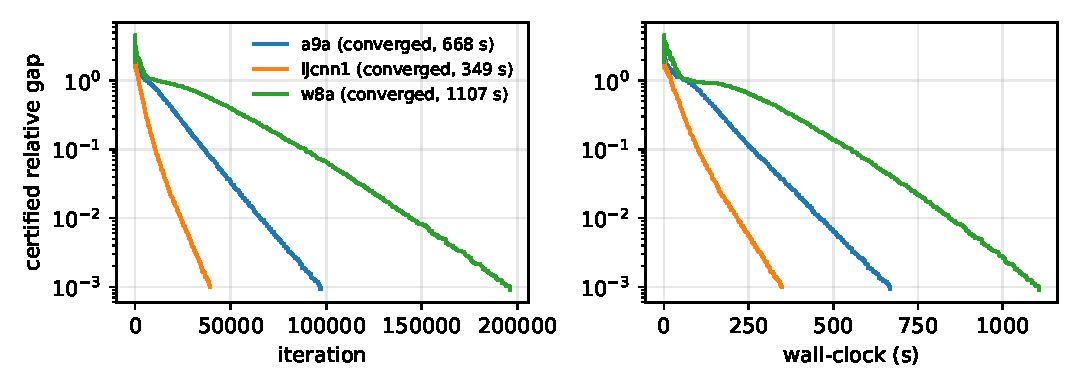
\includegraphics[width=\linewidth]{figs/fig_realdata_trace.pdf}
\caption{Certified relative gap of ETA on a9a, w8a and ijcnn1 ($L_2$,
$C=0.1$, uncapped, seed 0), versus iteration and wall-clock: linear-rate
convergence in the dense-support regime, reaching the certified
$10^{-3}$ in $349$--$1{,}107$\,s against the $600$\,s cap of
Table~\ref{tab:l2}.}\label{fig:trace}
\end{figure}

\paragraph{Hardware and protocol.} One dedicated 32-vCPU Intel Xeon
2.6\,GHz cloud VM, 122\,GB RAM, Linux, Python 3.12, NumPy 2.4 with
OpenBLAS 0.3.31, \texttt{OMP\_NUM\_THREADS=1}, no other load.
Table~\ref{tab:kreal} runs one configuration at a time in a fresh
process; Tables~\ref{tab:diag} and~\ref{tab:assump} run their twenty
configurations one after the other in a single process; the $L_2$
battery (Table~\ref{tab:l2}) ran four single-threaded cells at a time;
the synthetic tables, the screening and $n$-scaling experiments and the
uncapped traces ran one process at a time; Tables~\ref{tab:regime}
and~\ref{tab:bpcg} ran as up to 19 concurrent single-threaded processes
(the regime battery's 12 workers together with the BPCG,
LIBSVM-precomputed and ablation runs), and the isolated reruns of
their ETA and BPCG configurations in Table~\ref{tab:kreal} reproduce
those ratios; their SMO and LIBSVM columns were not rerun in isolation.
Five seeds unless stated, $t$-based 95\% intervals over seeds.
Concurrent load can manufacture ratios: under the 19-process load
guarded $k{=}1$ appeared $1.3\times$ faster than MDM on gisette, a tie
in isolation, and the gisette column time itself moved by $\pm15\%$
between three isolated runs of the same trajectory
(\texttt{results/step\_profile\{,2,3\}.json}); only ratios whose
intervals separate, and exceed that variation, are read as results.

\begin{table}[htbp]\centering\scriptsize\setlength{\tabcolsep}{4pt}
\caption{$L_2$ soft-margin battery: five seeds, 600\,s per solver for
ETA and our SMO (our own
implementation; LIBSVM does not solve this objective), LIBLINEAR
at tolerance $10^{-6}$ (Section~\ref{app:details}) with no cap; released
code, four single-threaded cells at a time on the 32-vCPU machine;
mean $\pm$ 95\% CI, which on the fixed-split datasets (all but
covtype) measures timing noise only. ``cap'' = timed out in every
seed; ETA's certified relative gap is reported at its stopping point
(mean [min, max]); accuracies are those of the returned
iterate.}\label{tab:l2}
\begin{tabular}{llrrrll}
\toprule
dataset ($n+m$ / $d$) & $C$ & ETA (s) & SMO (s) & LIBLINEAR (s) & ETA gap at stop & acc.\ ETA / SMO / LIBLINEAR \\
\midrule
gisette (6,000 / 5,000) & 0.1 & $30.0\pm3.6$ & $212\pm26$ & $462\pm70$ & $9\times10^{-4}$ & .981 / .981 / .981 \\
 & 1 & $29.6\pm3.0$ & $212\pm24$ & $3{,}060\pm491$ & $10\times10^{-4}$ & .981 / .981 / .981 \\
 & 10 & $28.3\pm2.9$ & $209\pm26$ & $5{,}031\pm337$ & $10\times10^{-4}$ & .981 / .981 / .977 \\
\midrule
a9a (32,561 / 123) & 0.1 & cap & cap & $2.6\pm0.6$ & 0.0045 [0.0037, 0.0060] & .850 / .850 / .849 \\
 & 1 & cap & cap & $3.2\pm0.9$ & 0.78 [0.75, 0.83] & .823 / .801 / .849 \\
 & 10 & cap & cap & $1.4\pm0.4$ & 1.2 [1.2, 1.2] & .505 / .768 / .849 \\
ijcnn1 (49,990 / 22) & 0.1 & $418\pm23$ & $200\pm14$ & $0.2\pm0.0$ & $10\times10^{-4}$ & .918 / .918 / .918 \\
 & 1 & cap & cap & $0.2\pm0.1$ & 0.29 [0.21, 0.36] & .923 / .918 / .918 \\
 & 10 & cap & cap & $0.1\pm0.0$ & 1.2 [1.2, 1.2] & .601 / .900 / .918 \\
w8a (49,749 / 300) & 0.1 & cap & cap & $14.2\pm3.5$ & 0.16 [0.08, 0.24] & .987 / .986 / .987 \\
 & 1 & cap & cap & $11.9\pm0.7$ & 0.92 [0.92, 0.93] & .895 / .978 / .987 \\
 & 10 & cap & cap & $14.6\pm0.9$ & 1.6 [1.5, 1.7] & .967 / .972 / .987 \\
covtype (100,000 / 54) & 0.1 & cap & cap & $22.5\pm21.2$ & 1.0 [1.0, 1.0] & .572 / .701 / .756 \\
 & 1 & cap & cap & $4.3\pm2.3$ & 1.1 [1.0, 1.1] & .537 / .545 / .756 \\
 & 10 & cap & cap & $3.7\pm1.1$ & 1.3 [1.3, 1.6] & .502 / .515 / .756 \\
\bottomrule
\end{tabular}
\end{table}

\paragraph{Reference solver in the KL2 cells.} The hinge-loss
\texttt{SVC(rbf, C=1)}, a different objective, took $4.4\pm0.6$ (a9a),
$3.1\pm0.1$ (covtype), $63.3\pm13.8$ (gisette), $1.0\pm0.1$ (ijcnn1) and
$2.7\pm0.7$\,s (w8a) in the run of Table~\ref{tab:regime}, with test accuracies $0.789$, $0.783$, $0.977$,
$0.950$ and $0.975$, within one point of the $L_2$ solutions and on
either side of them.

\paragraph{Step ablation, blocks and shrinking (synthetic).} Iteration
counts at $\varepsilon=10^{-6}$ on single instances from the
development log (\texttt{src/zigzag\_bench.py}; not part of the
rerun driver): $d{=}30$, $n{=}200$:
toward $158{,}941$, midpoint $148{,}996$, away $106$, pairwise $181$;
$d{=}100$, $n{=}1{,}000$: toward and midpoint fail within $300{,}000$,
away $15{,}886$, pairwise $3{,}921$. At the working tolerance $10^{-3}$
the pairwise/away gain over the midpoint heuristic of
\citet{gupta2026} is about $11\%$ on those instances. Block transfers
cut iterations $3$--$25\times$ relative to single MDM (e.g.\
$43{,}486\to3{,}001$ at $k{=}16$ on a dense-support $L_2$ instance at
$d{=}1{,}000$, Table~\ref{tab:kabl})
and are the only configuration that reaches the certified tolerance on
MNIST odd-vs-even within the iteration cap of that benchmark.
Figure~\ref{fig:shrink} shows the screening
speed-ups and Figure~\ref{fig:final} the consolidated comparison
(\texttt{src/final\_benchmark.py}), five trials per class (mean $\pm$
95\% CI). Its ``optimised'' configuration is $k{=}16$ with screening on
the hard-margin classes, $k{=}32$ on the $L_2$ class and $k{=}8$ on
MNIST; ``single MDM'' is the toward-step algorithm of
\citet{gupta2026} on the hard-margin rows and single MDM on the others,
both with a $2\times10^5$-iteration cap; our SMO there runs with a
$300$\,s cap and a two-row cache. On the four hard-margin
classes the optimised solver is $1.1$--$1.2\times$ faster than LIBSVM
on average, with overlapping intervals ($0.63\pm0.04$ vs
$0.75\pm0.15$\,s at $d{=}1{,}000$; $17.9\pm1.6$ vs $20.6\pm3.7$\,s at
$d{=}10{,}000$; $0.72\pm0.13$ vs $0.80\pm0.18$\,s at
$\varepsilon{=}10^{-5}$, where the toward-step configuration fails to
converge in every trial; RBF $2.33\pm0.06$ vs $2.50\pm0.12$\,s); on
the synthetic $L_2$ margin ($d{=}1{,}000$, $C{=}1$) it ties LIBLINEAR
($20.7\pm9.7$ vs $19.4\pm4.4$\,s); on MNIST odd-vs-even it is
$2.7\times$ slower ($172\pm20$ vs $63\pm22$\,s; single MDM does not
converge within its cap) and on the $\nu$-SVM $1.7\times$ slower ($61.0\pm5.0$ vs
NuSVC's $36.5\pm5.6$\,s). Distances agree within tolerance on every
row. On the four classes where single MDM also converges, blocks and
guard change wall-clock by $0.9$--$1.2\times$; their clear wins are the
two classes (tight tolerance, MNIST) where single MDM does not converge
within the cap.

\begin{table}[h]\centering\scriptsize
\caption{Two-sided schedules on the synthetic instances of this appendix ($n{=}5{,}000$ per class, $k{=}16$): the unconditional $V$-then-$W$ order used for the batteries versus the schedule of Lemma~\ref{lem:twosided} (larger-gap side first, second side skipped after a drop). Drop steps and skipped second-side steps are counted over the run.}\label{tab:sched}
\begin{tabular}{lllrrrr}\toprule
instance & schedule & time (s) & iterations & drops & skips & distance \\\midrule
hard margin, $d{=}1000$, $\varepsilon{=}10^{-5}$ & unconditional & 0.7 & 16 & 0 & 0 & 55.339365 \\
hard margin, $d{=}1000$, $\varepsilon{=}10^{-5}$ & Lemma~\ref{lem:twosided} & 0.7 & 16 & 0 & 0 & 55.339365 \\
\midrule
$L_2$ overlap, $d{=}100$, $C{=}1$ & unconditional & 22.2 & 12,311 & 785 & 0 & 0.078400 \\
$L_2$ overlap, $d{=}100$, $C{=}1$ & Lemma~\ref{lem:twosided} & 18.7 & 10,701 & 599 & 316 & 0.078400 \\
\midrule
$L_2$ overlap, $d{=}1000$, $C{=}1$ & unconditional & 11.5 & 2,901 & 182 & 0 & 0.578143 \\
$L_2$ overlap, $d{=}1000$, $C{=}1$ & Lemma~\ref{lem:twosided} & 12.0 & 3,001 & 180 & 121 & 0.578143 \\
\bottomrule
\end{tabular}\end{table}

\begin{table}[h]\centering\scriptsize
\caption{Block-size ablation on the same instances (current code): single MDM ($k{=}1$) versus blocks of $k$ transfers. Iterations fall with $k$; wall-clock does not fall in proportion, because each block iteration touches more columns.}\label{tab:kabl}
\begin{tabular}{lrrrrr}\toprule
instance & $k$ & time (s) & iterations & columns & drops \\\midrule
hard margin, $d{=}1000$, $\varepsilon{=}10^{-5}$ & 1 & 0.6 & 301 & 104 & 0 \\
hard margin, $d{=}1000$, $\varepsilon{=}10^{-5}$ & 4 & 0.5 & 36 & 103 & 0 \\
hard margin, $d{=}1000$, $\varepsilon{=}10^{-5}$ & 16 & 0.5 & 16 & 103 & 0 \\
hard margin, $d{=}1000$, $\varepsilon{=}10^{-5}$ & 32 & 0.6 & 16 & 109 & 0 \\
\midrule
$L_2$ overlap, $d{=}100$, $C{=}1$ & 1 & 16.6 & 72,546 & 1,345 & 0 \\
$L_2$ overlap, $d{=}100$, $C{=}1$ & 4 & 21.8 & 24,606 & 1,632 & 416 \\
$L_2$ overlap, $d{=}100$, $C{=}1$ & 16 & 20.0 & 10,701 & 2,404 & 599 \\
$L_2$ overlap, $d{=}100$, $C{=}1$ & 32 & 24.3 & 7,606 & 3,076 & 305 \\
\midrule
$L_2$ overlap, $d{=}1000$, $C{=}1$ & 1 & 22.7 & 43,486 & 1,242 & 0 \\
$L_2$ overlap, $d{=}1000$, $C{=}1$ & 4 & 18.3 & 10,071 & 1,330 & 177 \\
$L_2$ overlap, $d{=}1000$, $C{=}1$ & 16 & 12.7 & 3,001 & 1,348 & 180 \\
$L_2$ overlap, $d{=}1000$, $C{=}1$ & 32 & 12.0 & 1,741 & 1,396 & 170 \\
\bottomrule
\end{tabular}\end{table}


\begin{table}[htbp]\centering\scriptsize
\caption{LIBLINEAR on gisette at its default tolerance ($10^{-4}$)
versus the matched tolerance ($10^{-6}$) of Table~\ref{tab:l2}; five
seeds. ETA's certified primal is $0.14835$ / $0.14893$ / $0.14899$ at
$C=0.1$ / $1$ / $10$, reached in $28$--$30$\,s with test accuracy
$0.981$.}\label{tab:libdef}
\begin{tabular}{lrrrlr}\toprule
$C$ & tol & time (s) & iterations & primal (vs certified) & accuracy \\\midrule
0.1 & $10^{-4}$ & $51\pm1$ & 363 & 0.15648 ($+5.5\%$) & .978 \\
0.1 & $10^{-6}$ & $462\pm70$ & 2,434 & 0.14835 ($+0.0\%$) & .981 \\
1 & $10^{-4}$ & $4.3\pm0.1$ & 10 & 0.18427 ($+24\%$) & .974 \\
1 & $10^{-6}$ & $3{,}060\pm491$ & 18,063 & 0.14900 ($+0.05\%$) & .981 \\
10 & $10^{-4}$ & $3.5\pm0.1$ & 8 & 0.18487 ($+24\%$) & .973 \\
10 & $10^{-6}$ & $5{,}031\pm337$ & 35,411 & 0.15663 ($+5.1\%$) & .977 \\
\bottomrule\end{tabular}\end{table}

\begin{table}[htbp]\centering\scriptsize
\caption{Time to $1\%$ of the optimum, seed-0 traces. The ETA columns
measure \emph{dual} progress and LIBLINEAR's column \emph{primal}
progress, so this is not a matched primal comparison (the primal of
ETA's returned $(w,b)$ is not recorded in the traces). For ETA the
certified dual value $2/\UB_t^2$ increases to the optimum,
so $s_t=1-(2/\UB_t^2)/P^*$ with $P^*$ the best known primal (the lower
of LIBLINEAR's $10^{-6}$ value and ETA's certified value); ``certified
$1\%$'' is the first time the certificate itself proves
$1-\LB_t^2/\UB_t^2\le1\%$. ETA's a9a, w8a and ijcnn1 times are from
the uncapped runs of Figure~\ref{fig:trace} (\texttt{src/time\_to\_tol.py}).
The LIBLINEAR entries are the five-seed mean times of the matched
$10^{-6}$ run of Table~\ref{tab:l2}, an upper bound on its time to
$1\%$ (the sweep that would give the exact value is listed in
Section~\ref{sec:limits}); ``none'' means that neither $10^{-4}$ nor
$10^{-6}$ reaches $1\%$. On the
remaining cells ETA is not within $1\%$ at the 600\,s cap
($s=11$--$99\%$).}\label{tab:t1}
\setlength{\tabcolsep}{3.5pt}
\begin{tabular}{llrrrrrl}\toprule
dataset & $C$ & $P^*$ & ETA $1\%$ & ETA $0.1\%$ & cert.\ $1\%$ & cert.\ $10^{-3}$ & LIBLINEAR $1\%$ \\\midrule
gisette & 0.1 & 0.14835 & 30 s & 31 s & 31 s & 32 s & $\le462$ s (tol $10^{-6}$) \\
gisette & 1 & 0.14893 & 30 s & 31 s & 32 s & 33 s & $\le3{,}060$ s (tol $10^{-6}$) \\
gisette & 10 & 0.14899 & 24 s & 26 s & 26 s & 27 s & none at $10^{-4}$ or $10^{-6}$ \\
\midrule
a9a & 0.1 & 687.07 & 274 s & 385 s & 524 s & 668 s & $\le2.6$ s (tol $10^{-6}$) \\
w8a & 0.1 & 108.80 & 589 s & 764 s & 929 s & 1,107 s & $\le14$ s (tol $10^{-6}$) \\
ijcnn1 & 0.1 & 550.61 & 108 s & 172 s & 256 s & 349 s & $\le0.2$ s (tol $10^{-6}$) \\
\bottomrule\end{tabular}\end{table}





\begin{figure}[htbp]\centering
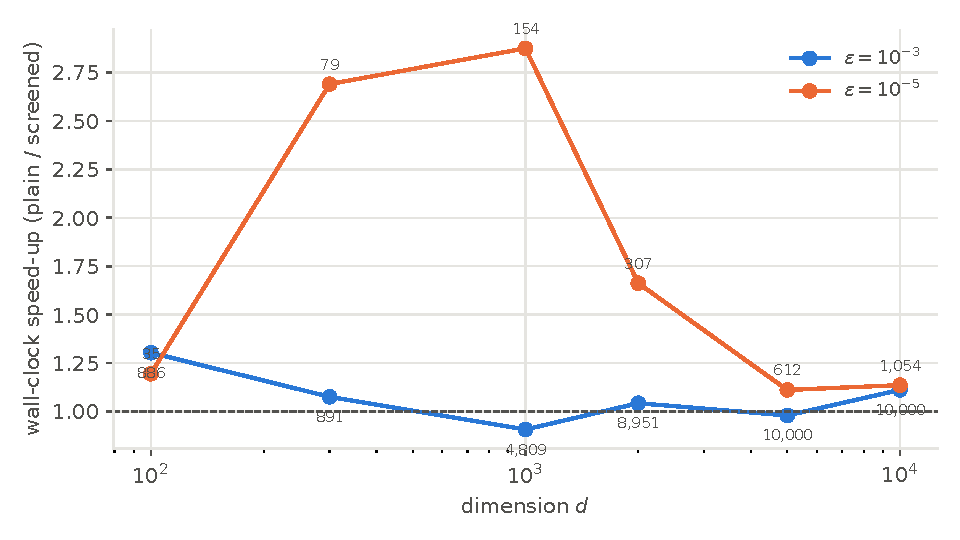
\includegraphics[width=.7\linewidth]{figs/fig_shrink.pdf}
\caption{Safe screening on the separated synthetic protocol
($n{=}10{,}000$, two trials): wall-clock speed-up of screening versus
dimension at $\varepsilon=10^{-3}$ and $10^{-5}$; labels are surviving
points of $10{,}000$. Made with the toward-step solver of the
development phase (\texttt{src/shrink\_benchmark.py}); the rule and its
activation do not depend on the step, and Table~\ref{tab:screen} gives
the released solver on real data.}\label{fig:shrink}
\end{figure}

\begin{figure}[htbp]\centering
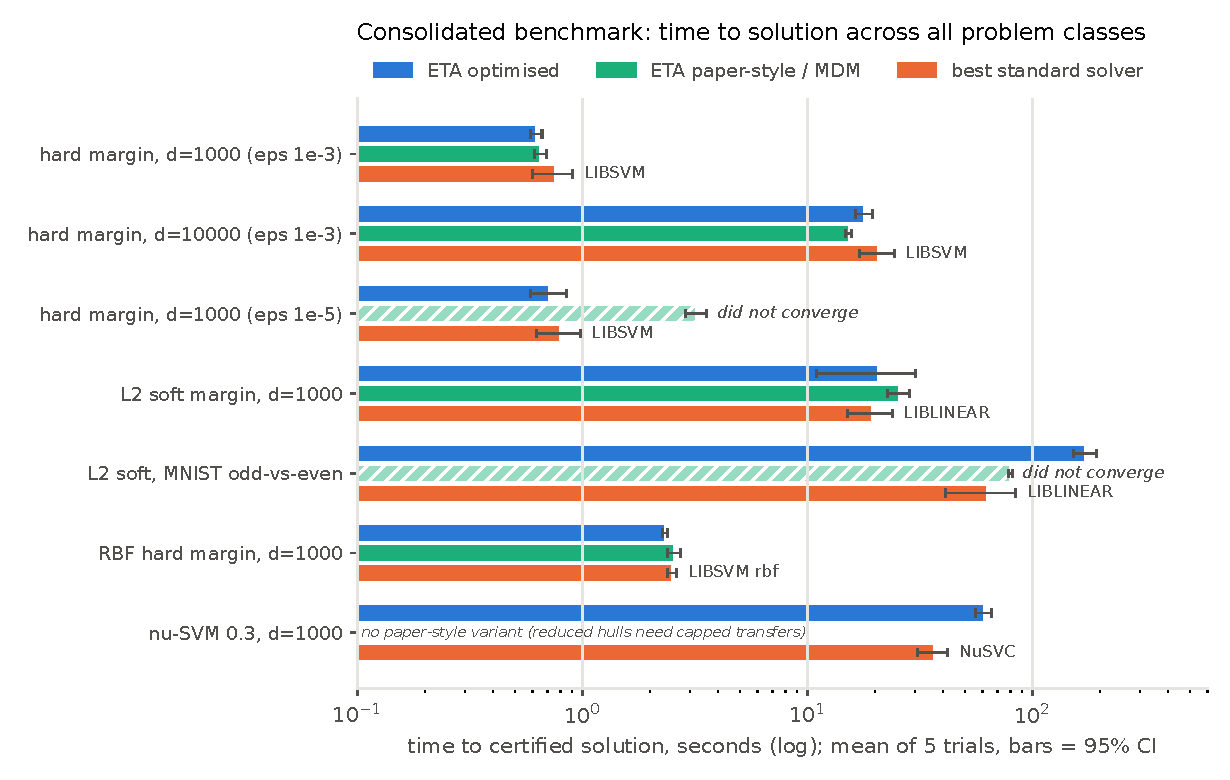
\includegraphics[width=.78\linewidth]{figs/fig_final.pdf}
\caption{Time to certified solution on seven problem classes: the
optimised configuration vs the toward-step or single-MDM configuration
vs the best standard solver per class (settings in
Section~\ref{app:details}); five trials per class, mean with 95\% CI.
The $\nu$-SVM row has no toward-step bar because the algorithm of
\citet{gupta2026} has no reduced-hull variant (reduced hulls need
capped transfers).}\label{fig:final}
\end{figure}

\subsection{Numerical verification of the analysis}\label{app:num}
Lemma~\ref{lem:block} was checked on $4{,}000$ random ensembles
including heavily clipped and boundary cases (worst slack at machine
precision); Proposition~\ref{prop:orth} on $500$ near-orthogonal
ensembles; Lemma~\ref{lem:gapid} to $10^{-9}$ at arbitrary iterates;
Lemma~\ref{lem:twosided} on instrumented two-sided runs (no drop
iteration added a support index, and every non-drop iteration met the
gain bound with $M$ replaced by the computable upper bound
$\operatorname{diam}V+\operatorname{diam}W$); and Theorem~\ref{thm:activation} on instances whose optimal
face was computed by the SLSQP reference: at every activating round all
zero-weight non-face points were screened, and the final working set
lay in the union of the optimal face and the final support. Over $5{,}000$ instrumented live
block steps none increased the objective. All checks are test files in
the released code.

\section{When does aggregation pay: measurements}\label{sec:pay-meas}

\subsection{Step ablation on real data}\label{sec:meas-kreal}
Table~\ref{tab:kreal} separates the three effects the batteries of
Section~\ref{sec:exp} mix: the guard and away fallback (guarded $k{=}1$
against plain MDM), aggregation ($k{=}16$ and the adaptive size of
Section~\ref{sec:adaptive} against guarded $k{=}1$), and the
comparison with BPCG, all in isolated runs with a time split. Two
effects separate. The guard and away fallback alone cut plain pairwise
FW's iterations $1.4$--$2.7\times$ and its time by at most $1.3\times$
(a tie on gisette and ijcnn1); aggregation cuts iterations a further
$3.8$--$7.0\times$, which buys wall-clock only where per-iteration
$O(n)$ work, not column computation, dominates: $1.8$--$2.4\times$
over guarded $k{=}1$ on the four kernel cells ($3.8$--$6.1\times$ over
BPCG) and nothing on gisette.

\begin{table}[htbp]\centering\scriptsize\setlength{\tabcolsep}{3.5pt}
\caption{Step ablation on real data with a time split, isolated runs
(\texttt{src/step\_profile.py}: three seeds, each configuration alone
in its own process on an otherwise idle machine, with the final code):
the gisette $L_2$
margin ($C{=}1$, $d{=}5{,}000$) and the four kernel $L_2$ cells of
Table~\ref{tab:regime}. MDM is plain
pairwise FW (single transfers, no guard, no fallback, the same
prioritised receiver search and schedule as the other rows); guarded $k{=}1$
is Algorithm~\ref{alg:block} with a single pair (guard and case-(b)
fallback active); auto is the adaptive block size of
Section~\ref{sec:adaptive} (median $k$ over the run given); BPCG as in
Table~\ref{tab:bpcg}. Split of the ETA time: scan = the score scan and
pair selection; col = Gram or kernel column computation; step = the
step itself (block assembly, guard, line search, cache and score
update); rest = certificate and bounds. Drops = away fallbacks that
removed a support index. Every run converged to the certified gap with
identical distance and accuracy per dataset and seed. Peak resident
memory: $0.74$\,GB on gisette, $0.48$--$0.93$\,GB for ETA and
$0.66$--$1.29$\,GB for BPCG on the kernel cells. The gisette column
time varied by $\pm15\%$ between three isolated runs of the same
trajectory on the same machine ($26$--$35$\,s;
\texttt{results/step\_profile\{,2,3\}.json}), more than the $8\%$
that separates its fastest and slowest rows here, so its rows should be
read as a tie.}\label{tab:kreal}
\begin{tabular}{llrrrrrrrrr}\toprule
instance & step & $k$ & time (s) & scan & col & step & rest & iterations & columns & drops \\\midrule
gisette $L_2$ & MDM & 1 & $29.4\pm0.2$ & 0.2 & 26.0 & 1.0 & 2.1 & 4,946 & 1,300 & 0 \\
gisette $L_2$ & guarded & 1 & $30.1\pm0.3$ & 0.2 & 26.6 & 1.8 & 1.5 & 3,471 & 1,334 & 82 \\
gisette $L_2$ & block & 16 & $31.9\pm0.5$ & 0.1 & 29.7 & 1.7 & 0.4 & 831 & 1,480 & 301 \\
gisette $L_2$ & auto & 9 & $30.9\pm1.4$ & 0.1 & 28.8 & 1.6 & 0.5 & 986 & 1,451 & 194 \\
gisette $L_2$ & BPCG & --- & $29.8\pm0.5$ & & & & & 10,470 & 1,322 & 87 \\
\midrule
ijcnn1 kernel $L_2$ & MDM & 1 & $10.3\pm0.5$ & 1.3 & 0.9 & 2.9 & 5.2 & 12,796 & 4,520 & 0 \\
ijcnn1 kernel $L_2$ & guarded & 1 & $9.7\pm0.4$ & 0.8 & 0.8 & 4.5 & 3.6 & 6,118 & 4,514 & 14 \\
ijcnn1 kernel $L_2$ & block & 16 & $5.3\pm0.8$ & 0.2 & 0.8 & 3.3 & 1.0 & 1,396 & 4,590 & 98 \\
ijcnn1 kernel $L_2$ & auto & 8 & $4.7\pm0.6$ & 0.3 & 0.7 & 2.6 & 1.1 & 1,734 & 4,570 & 75 \\
ijcnn1 kernel $L_2$ & BPCG & --- & $19.9\pm2.2$ & & & & & 18,034 & 4,512 & 19 \\
\midrule
w8a kernel $L_2$ & MDM & 1 & $8.8\pm0.8$ & 0.9 & 2.8 & 2.2 & 2.9 & 11,461 & 3,587 & 0 \\
w8a kernel $L_2$ & guarded & 1 & $7.3\pm1.2$ & 0.4 & 2.7 & 2.7 & 1.4 & 4,243 & 3,581 & 8 \\
w8a kernel $L_2$ & block & 16 & $4.0\pm0.2$ & 0.1 & 2.4 & 1.2 & 0.3 & 603 & 3,591 & 50 \\
w8a kernel $L_2$ & auto & 10 & $3.8\pm0.2$ & 0.1 & 2.3 & 1.1 & 0.3 & 756 & 3,590 & 40 \\
w8a kernel $L_2$ & BPCG & --- & $17.5\pm2.0$ & & & & & 12,342 & 3,577 & 12 \\
\midrule
a9a kernel $L_2$ & MDM & 1 & $31.5\pm1.6$ & 3.4 & 4.5 & 7.3 & 16.4 & 22,901 & 7,607 & 0 \\
a9a kernel $L_2$ & guarded & 1 & $24.2\pm2.1$ & 1.9 & 3.9 & 9.7 & 8.8 & 9,879 & 7,611 & 27 \\
a9a kernel $L_2$ & block & 16 & $10.0\pm0.5$ & 0.3 & 3.8 & 4.2 & 1.7 & 1,489 & 7,616 & 35 \\
a9a kernel $L_2$ & auto & 13 & $10.0\pm0.5$ & 0.4 & 3.7 & 4.0 & 1.9 & 1,641 & 7,607 & 26 \\
a9a kernel $L_2$ & BPCG & --- & $60.7\pm1.2$ & & & & & 28,653 & 7,605 & 24 \\
\midrule
covtype kernel $L_2$ & MDM & 1 & $39.5\pm1.4$ & 4.4 & 2.9 & 9.6 & 22.6 & 26,756 & 9,069 & 0 \\
covtype kernel $L_2$ & guarded & 1 & $33.4\pm2.2$ & 2.6 & 2.5 & 13.7 & 14.6 & 12,544 & 9,069 & 12 \\
covtype kernel $L_2$ & block & 16 & $17.4\pm0.5$ & 0.9 & 2.5 & 9.4 & 4.6 & 3,336 & 9,074 & 26 \\
covtype kernel $L_2$ & auto & 7 & $16.8\pm1.7$ & 1.0 & 2.4 & 7.9 & 5.5 & 4,154 & 9,071 & 19 \\
covtype kernel $L_2$ & BPCG & --- & $85.3\pm4.5$ & & & & & 38,422 & 9,065 & 15 \\
\bottomrule\end{tabular}\end{table}

The guarded single pair already halves the iterations of plain MDM on
ijcnn1 ($1.4\times$ on gisette): the drop steps it takes (on $0.1$--$2.4\%$
of its iterations) are what plain pairwise FW replaces by capped
swaps. Blocks then cut iterations a further $3.8$--$7.0\times$
(isolated seed-0 runs at $k{=}4$ are in Table~\ref{tab:diag}: within
$31\%$ of $k{=}16$ in time on every cell). Away fallbacks that drop an index occur on
$0.1$--$36\%$ of guarded iterations, and their share grows with $k$:
larger blocks add more indices per iteration, and the drops remove
them. The time split says where fewer iterations buy time. On gisette,
$88$--$93\%$ of every configuration's time is Gram-column computation
($O(nd)$ per new receiver, $d{=}5{,}000$), so MDM, guarded $k{=}1$,
block $k{=}16$, the adaptive size and BPCG all lie within $8\%$ of one
another at $29$--$32$\,s, inside the between-run variation of the
column time. On ijcnn1 the columns cost
about $1$\,s and the rest is per-iteration $O(n)$ work: the score
update and line search inside the step, the certificate in the
remainder, and least of all the scan itself. That work falls with the
iteration count, though not in proportion, because a block step updates
the scores with up to $k'$ columns; the net effect on ijcnn1 is
$1.9\times$ over MDM and $3.8\times$ over BPCG at $k{=}16$, and
$2.2\times$ and $4.2\times$ with the adaptive size, which settles at
$k{=}7$--$8$, the $k^*$ of Section~\ref{sec:pay-meas}; the other three
kernel cells behave alike (Table~\ref{tab:kreal}).

\begin{table}[htbp]\centering\scriptsize
\caption{BPCG \citep{tsuji2022} versus block ETA ($k{=}16$) on the same
objective with the same certificate ($\varepsilon{=}10^{-3}$), the same
column cache and the same 600\,s cap (\texttt{src/bpcg\_baseline.py},
solver \texttt{src/bpcg.py}); three seeds,
run concurrently with Table~\ref{tab:regime}; Table~\ref{tab:kreal}
gives the isolated reruns. Every cell converged; distances agree per
cell to five digits and test accuracies to $10^{-4}$. Columns are
kernel or Gram columns computed; drops count BPCG's capped
local steps and ETA's away drops.}\label{tab:bpcg}
\begin{tabular}{llrrrr}\toprule
cell & solver & time (s) & iterations & columns & drops \\\midrule
gisette $L_2$, $C{=}1$ & BPCG & $34.2\pm20.4$ & 10,470 & 1,322 & 87 \\
gisette $L_2$, $C{=}1$ & ETA & $34.3\pm15.0$ & 831 & 1,480 & 301 \\
\midrule
gisette KL2 & BPCG & $213\pm28$ & 8,702 & 3,641 & 3 \\
gisette KL2 & ETA & $83.9\pm19.0$ & 251 & 3,653 & 4 \\
w8a KL2 & BPCG & $22.3\pm5.8$ & 12,342 & 3,577 & 12 \\
w8a KL2 & ETA & $5.0\pm2.2$ & 603 & 3,591 & 50 \\
a9a KL2 & BPCG & $65.4\pm5.7$ & 28,653 & 7,605 & 24 \\
a9a KL2 & ETA & $11.7\pm2.2$ & 1,489 & 7,616 & 35 \\
covtype KL2 & BPCG & $90.6\pm11.2$ & 38,422 & 9,065 & 15 \\
covtype KL2 & ETA & $20.3\pm1.1$ & 3,336 & 9,074 & 26 \\
ijcnn1 KL2 & BPCG & $20.2\pm1.6$ & 18,034 & 4,512 & 19 \\
ijcnn1 KL2 & ETA & $5.9\pm1.1$ & 1,396 & 4,590 & 98 \\
\bottomrule\end{tabular}\end{table}

BPCG here is the blended pairwise step of \citet{tsuji2022} on the
$nm$ product atoms $v_i-w_j$ of $Z$, with product-atom capacities, the
separable LMO of Lemma~\ref{lem:sep}, exact line searches and the
certificate of Lemma~\ref{lem:gapid}; its scores are maintained from
the same cached columns, so column counts are comparable, but its
active set is a Python-level dictionary over product atoms, and on that
parametrisation it needs $1.1$--$2.1\times$ more iterations than even
plain MDM with side transfers (gisette $10{,}470$ vs $4{,}946$; ijcnn1
$18{,}034$ vs $12{,}796$). The $11$--$35\times$ iteration ratio and the
$2.5$--$5.6\times$ wall-clock ratio against block ETA therefore compare
parametrisation and implementation as well as step rules; a BPCG on the
side-transfer parametrisation is listed in Section~\ref{sec:limits}.
The block's fewer scans buy time where scans dominate (KL2) and nothing
where columns do (gisette $L_2$).

\subsection{Per-step measurements}\label{sec:meas}

Every quantity in Proposition~\ref{prop:ratio}, the cost model and
Theorem~\ref{thm:ident} was recorded on the five real cells of
Table~\ref{tab:regime} (gisette $L_2$ and the kernel $L_2$ cells of
ijcnn1, w8a, a9a and covtype, seed 0; \texttt{src/block\_diagnostics.py}, one process at a time on an
otherwise idle machine, $k\in\{1,4,16,32\}$). At every block step the
solver logs $\Delta_B$, $\Delta_1$, $Q$, $\chi$, the candidate taken,
the capped pairs, the column misses, the support size and a time split
of the step next to a dry-run timing of the single MDM update from the
same state. Table~\ref{tab:diag} fits the model per cell:
$\hat\eta=(\chi-1)/(k'-1)$ (median over the block calls with pair 1
uncapped; a \emph{block call} is one side's execution of
Algorithm~\ref{alg:block}, up to two per iteration), $a$ and $b$ by
least squares of the non-column time per iteration on $k$,
$c_{\mathrm{col}}$ as column time per column.

\begin{table}[t]\centering\scriptsize\setlength{\tabcolsep}{4pt}
\caption{The timing model fitted per cell (seed 0; the twenty
configurations run one after the other in a single process with the
per-step instrumentation on, which adds $5$--$34\%$ to the times of
Table~\ref{tab:kreal}; the coefficients describe these instrumented
runs). $\hat\eta$ is the median over $k\in\{4,16,32\}$; the $k=16$ and
$k=32$ estimates agree within $0.01$ and the $k=4$ estimate within
$0.04$ of them (gisette $0.04/0.08/0.07$, w8a $0.20/0.17/0.16$). $k^*$
from \eqref{eq:kstar} with $\hat\eta$ in place of $\eta$. Times for $k=1/4/16/32$; ``column share'' is the
fraction of the $k{=}16$ run spent computing columns; the last column is
the speed-up of the best $k$ over the guarded single pair.}\label{tab:diag}
\begin{tabular}{lrrrrrlrr}\toprule
cell & $\hat\eta$ & $a$ (ms) & $b$ (ms) & $c_{\mathrm{col}}$ (ms) & $k^*$ & time (s), $k=1/4/16/32$ & column share & best $k$ vs $k{=}1$ \\\midrule
% rows generated by src/block_diag_fig.py --inp results/block_diag3.json
gisette $L_2$ & 0.07 & 1.3 & 0.080 & 21.30 & 14 & 33.0 / 29.2 / 33.9 / 38.0 & 93\% & 1.1$\times$ (4) \\
ijcnn1 KL2 & 0.26 & 1.7 & 0.098 & 0.23 & 7 & 11.6 / 6.1 / 6.1 / 7.6 & 17\% & 1.9$\times$ (4) \\
w8a KL2 & 0.17 & 1.3 & 0.077 & 0.88 & 9 & 9.7 / 5.3 / 4.4 / 4.6 & 64\% & 2.2$\times$ (16) \\
a9a KL2 & 0.11 & 2.5 & 0.111 & 0.62 & 13 & 30.5 / 14.2 / 10.8 / 11.7 & 41\% & 2.8$\times$ (16) \\
covtype KL2 & 0.29 & 2.8 & 0.102 & 0.35 & 8 & 38.9 / 21.0 / 18.2 / 21.7 & 17\% & 2.1$\times$ (16) \\
\bottomrule\end{tabular}\end{table}

\begin{figure}[t]\centering
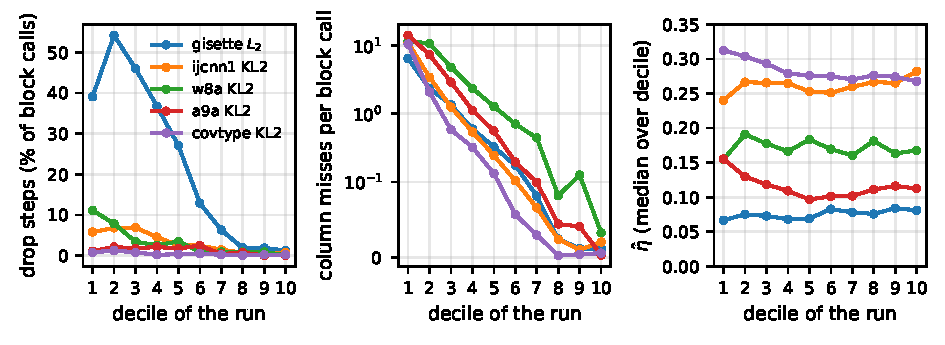
\includegraphics[width=\linewidth]{figs/fig_diag.pdf}
\caption{Along the run at $k=16$ (deciles of the iteration count, one
line per cell): fraction of block calls that are drops, column misses per
block call, and the effective correlation $\hat\eta$. Drops and misses
are paid while the support is built and become rare once it has
settled, the shape Theorem~\ref{thm:ident} describes; $\hat\eta$ is
constant along the run.}\label{fig:diag}
\end{figure}

Four facts follow.
\begin{itemize}\setlength\itemsep{0pt}
\item \emph{$\hat\eta$ is stable on each cell.} The effective
correlation does not move with $k$ nor along the run
(Figure~\ref{fig:diag}, right), although it is a statistic of the
iterates and the pairing rule rather than of the data alone; it is $0.07$ on
gisette, $0.11$ on a9a, $0.17$ on w8a, $0.26$ on ijcnn1 and $0.29$ on
covtype, and $0.001$ on the synthetic instance of
Table~\ref{tab:adaptive} at $d{=}1{,}000$. The mean relative pair gain
$Q/k'=(1/k')\sum_j\Delta_j/\Delta_1$ (median $Q$ over the run's block
calls with pair 1 uncapped, divided by the mean number of retained
pairs) is $0.92$--$0.98$ at $k=4$, $0.83$--$0.98$ at $k=16$ and
$0.78$--$0.88$ at $k=32$ (Table~\ref{tab:assump} lists the $k=16$
values): the useful progress beyond the leading pair is never the
limit, the loss to combination is. The measured gain ratios (median
$\max(\Delta_B,\Delta_1)/\Delta_1$ over the same calls: $3.4/6.9/7.5$ on
gisette and $2.1/2.8/3.0$ on ijcnn1 at $k=4/16/32$) follow
$k/(1+\hat\eta(k-1))$ within $35\%$; on ijcnn1 they saturate near
$1/\hat\eta=3.8$, on gisette they are still rising at $k=32$ ($7.5$
against $1/\hat\eta=14$).
\item \emph{$k^*$ is $7$--$14$ on every cell}, because $a/b$ is
$16$--$28$ throughout and $\hat\eta\in[0.07,0.29]$: a fixed block size
of $8$--$16$ is within $16\%$ of the best measured time on all five
cells ($k{=}16$ against the best size: $16\%$ on gisette, under $1\%$
elsewhere; $k{=}4$ is within $31\%$ of $k{=}16$ on every cell), so the
untuned $k=16$ of Section~\ref{sec:exp} never lost to another size by
more than that.
\item \emph{The wall-clock gain is bounded by the single pair's column
share.} The block cannot touch the column term of the timing model
($N_{\mathrm{cols}}$ varies by under $20\%$ across $k$ on every cell),
so no block size can beat the guarded single pair by more than the
reciprocal of the fraction of that run spent on columns ($T_1/T_{\mathrm{col}}$:
$1.1$ on gisette, $2.4$ on w8a, $5.5$ on a9a, $11$--$12$ on ijcnn1 and
covtype). The measured speed-ups are $1.1\times$ on gisette,
$2.2\times$ on w8a, $2.8\times$ on a9a and $1.9$--$2.1\times$ on ijcnn1
and covtype, where the iteration gain has saturated at $1/\hat\eta$
long before the column bound matters. (The share of the $k{=}16$ run
in the table is not a bound: w8a's $2.2\times$ exceeds $1/0.64$.) The
model's time predictions, $aT+b\sum_tk'_t+c_{\mathrm{col}}N_{\mathrm{cols}}$
with the fitted coefficients, are within $14\%$ of the measurements at
$k\le4$ and within $5\%$ on gisette at every $k$; at $k=16$--$32$ on
the kernel cells they are $24$--$50\%$ too high, because the runs need
fewer iterations than the one-state ratio predicts: the trajectory
effect is in the block's favour, and the model is conservative.
\item \emph{Drops are front-loaded} (Figure~\ref{fig:diag}, left). On
gisette at $k=16$ half of the block calls in the first three deciles are
drops and $1$--$2\%$ in the last three; the kernel cells show the same
shape at lower levels; nearly every case-(b) call is a drop, so the
best-of-four branch is rare. Column misses follow the same curve, so on
column-bound cells the whole column bill is paid during identification
whichever $k$ is used. Total drops per point of one class's final
support are $0.13/0.13/0.48/0.69$ on gisette and $0.003$--$0.10$ on the
kernel cells for $k=1/4/16/32$: growing with $k$, and an order of
magnitude more frequent on the sparse linear cell, where fresh
receivers of small weight become the worst donor at once. On a9a and
covtype the drop fraction is flat over the first six deciles rather
than front-loaded; the shape of Theorem~\ref{thm:ident} is clearest on
gisette, ijcnn1 and w8a.
\end{itemize}
\begin{table}[t]\centering\scriptsize
\caption{The theorem's assumptions against the measured mechanism at
$k=16$ (seed 0; \texttt{src/block\_diagnostics.py} on a second machine,
with iteration and drop counts identical to the runs of
Table~\ref{tab:diag}; its $\hat\eta$ differs from Table~\ref{tab:diag}
in the second decimal because it is the $k=16$ median alone rather than
the median over $k\in\{4,16,32\}$). Over the
block calls with every retained pair uncapped: median maximum absolute
pairwise cosine of the retained directions (the $\eta$ of
Proposition~\ref{prop:ratio}), median minimum relative pair gain (its
$\beta_{\mathrm{flat}}$), and the lower bound the proposition then
guarantees for the guarded ratio $\max(\Delta_B,\Delta_1)/\Delta_1$,
$(1+\beta_{\mathrm{flat}}(k'-1))/(1+\eta(k'-1))$ (column ``bound''); against
the effective correlation $\hat\eta$, the mean relative pair gain
$Q/k'$, the model ratio $k'/(1+\hat\eta(k'-1))$ and the measured median
of $\max(\Delta_B,\Delta_1)/\Delta_1$, the last three over the block
calls with pair 1 uncapped.}\label{tab:assump}
\begin{tabular}{lrrrrrrrr}\toprule
cell & all pairs uncapped & $\max|\cos|$ & $\beta_{\mathrm{flat}}$ & bound & $\hat\eta$ & $Q/k'$ & model & measured \\\midrule
gisette $L_2$ & 43\% & 0.33 & 0.53 & 1.5 & 0.08 & 0.98 & 7.4 & 6.9 \\
ijcnn1 KL2 & 73\% & 0.42 & 0.80 & 1.8 & 0.26 & 0.89 & 3.2 & 2.8 \\
w8a KL2 & 76\% & 0.33 & 0.77 & 2.1 & 0.17 & 0.88 & 4.4 & 3.6 \\
a9a KL2 & 89\% & 0.28 & 0.70 & 2.2 & 0.12 & 0.83 & 5.8 & 4.6 \\
covtype KL2 & 96\% & 0.42 & 0.82 & 1.8 & 0.28 & 0.91 & 3.0 & 2.7 \\
\bottomrule\end{tabular}\end{table}

\emph{The theorem's constants are not what the mechanism runs on.}
Table~\ref{tab:assump} records the assumptions of
Proposition~\ref{prop:ratio} on the real cells. The maximum pairwise
cosine is $0.28$--$0.42$ on every cell, so the $\eta$ of the proposition
does not distinguish the cells at all, whereas the effective correlation
$\hat\eta$ spans $0.07$--$0.29$ and does; the minimum relative gain is
$0.53$--$0.82$; and at $k=16$ only $43$--$96\%$ of the block calls have all
pairs uncapped, so the proposition applies to a minority of the calls on
gisette. The lower bound the proposition guarantees for the guarded
ratio from these constants is $1.5$--$2.2$, against measured medians of
$2.7$--$6.9$ (the bound is an inequality, so the gap is slack, not a
contradiction). The exact identity $Q/\chi$ evaluated on the same calls
gives $7.3/2.9/3.9/4.8/2.8$ against the measured $6.9/2.8/3.6/4.6/2.7$;
the ``model'' column, $k'/(1+\hat\eta(k'-1))$, which replaces $Q$ by
$k'$, is $7$--$26\%$ high. Both reproduce the measurement to within the
spread because they use the $\gamma$-weighted aggregate in which the
cross terms largely cancel, not the worst pair. The right reading of
Proposition~\ref{prop:ratio} is therefore its first, exact, half; the
$\eta$-diverse, $\beta_{\mathrm{flat}}$-flat bound is a worst case that real blocks beat
by a factor of $1.5$--$4.6$.

The measurements are from one seed per cell and the fits are
retrospective (the coefficients are estimated from the same four runs
they describe); the ratios they support (Tables~\ref{tab:kreal}
and~\ref{tab:bpcg}) are reproduced across three seeds in isolated runs,
and Section~\ref{sec:adaptive} is the prospective test. On the
identification mechanism the figure is consistent with
Theorem~\ref{thm:ident} but does not verify it: the theorem's thresholds
$H_{\mathrm{id}},H_{\mathrm w}$ lie below the stopping tolerance of
these runs, and late drops, though rare, do occur. Section~\ref{sec:ident-check}
tests the theorem where its constants can be computed.

\subsection{An adaptive block size}\label{sec:adaptive}

Every quantity in \eqref{eq:kstar} is observable while the solver runs:
$\chi$ is computed by the guard at every block step, so
$\hat\eta=(\chi-1)/(k'-1)$ costs nothing, and $a/b$ is a property of
the implementation ($16$--$28$ in Table~\ref{tab:diag}). The released
code therefore offers \texttt{block\_size='auto'}: every $50$ iterations
it sets $k$ to $\sqrt{(a/b)(1-\hat\eta)/\hat\eta}$, clipped to $[1,k_{\max}]$,
with $\hat\eta$ the median over the window's block steps with $k'>1$
(when fewer than five such steps exist, as at $k=1$, the rule doubles
$k$ to obtain a signal; a non-positive $\hat\eta$ is floored at $10^{-3}$
before the square root, which sends $k$ to $k_{\max}$), and halves $k$ instead when
more than $10\%$ of the window's block calls had their leading pair
capped (drops are outrunning the support). Guard and fallback are
untouched, so Theorem~\ref{thm:linear} applies with $k_{\max}$ in the
drop bound. The rule's form, its window, $k_{\max}=32$ and the ratio
$a/b=20$ were set from the analysis of the two pilot cells (gisette,
ijcnn1); on a run the rule reads only its own window's $\chi$ values,
never the per-cell $\hat\eta$ of Table~\ref{tab:diag}, which is a
retrospective median over three complete runs and enters nothing but
the fitted $k^*$ column of that table. We do not call the other three
cells a prospective test: the $k$-sweeps on w8a, a9a and covtype were
on disk before the rule was committed, and the repository cannot
establish that the constants were fixed without sight of them. They
are cells not used to set the constants, and the check is whether the
rule's wall-clock on them matches the fixed sizes run under the same
protocol (Table~\ref{tab:kreal}). It does: the rule settles at $k=10$,
$13$ and $7$ (the retrospectively fitted $k^*$ are $9$, $13$, $8$) and
takes $3.8\pm0.2$, $10.0\pm0.5$ and $16.8\pm1.7$\,s against
$4.0\pm0.2$, $10.0\pm0.5$ and $17.4\pm0.5$\,s for $k{=}16$, a tie
within CI on every cell, as it is on the two pilot cells ($k{=}9$ then
$15$ on gisette; $k{=}7$--$8$ on ijcnn1, $4.7\pm0.6$ against
$5.3\pm0.8$\,s). The rule's value is that it removes the parameter,
not that it beats a well-chosen fixed size. Table~\ref{tab:adaptive} tests it where
$\eta$ actually varies: synthetic $L_2$ instances ($n{=}2{,}000$ per
class, $C{=}1$) whose transfer directions decorrelate as the dimension
grows, so that $\hat\eta$ falls from $0.31$ at $d{=}20$ to below
$0.002$ at $d\ge300$. The rule tracks $k^*$ across two orders of
magnitude of $\hat\eta$ and is within $0.14$\,s ($14\%$) of the best
fixed size at $d{=}20$ and within $0.1$\,s elsewhere, the resolution of
these short single-seed runs.

\begin{table}[t]\centering\scriptsize
\caption{Adaptive block size on synthetic $L_2$ instances of varying
directional diversity (one process, seed 0, $a/b$ set to $20$,
$k_{\max}=32$). Times for guarded $k{=}1$ and fixed $k=4/16/32$; ``auto''
reports the size the rule settled on and its time.}\label{tab:adaptive}
\begin{tabular}{rrrrrrrr}\toprule
$d$ & $\hat\eta$ & $k^*$ & $k{=}1$ (s) & $k{=}4$ & $k{=}16$ & $k{=}32$ & auto: $k$, time (s) \\\midrule
20 & 0.31 & 7 & 1.3 & 1.0 & 1.1 & 1.3 & 6, 1.1 \\
50 & 0.10 & 13 & 2.1 & 1.2 & 1.0 & 1.3 & 12, 1.1 \\
100 & 0.03 & 24 & 3.5 & 1.8 & 1.1 & 1.2 & 24, 1.1 \\
300 & 0.00 & $>32$ & 1.7 & 0.7 & 0.4 & 0.4 & 32, 0.4 \\
1,000 & 0.00 & $>32$ & 1.5 & 0.9 & 0.7 & 0.7 & 32, 0.7 \\
\bottomrule\end{tabular}\end{table}

\subsection{Numerical check of Theorem~\ref{thm:ident}}\label{sec:ident-check}

The theorem's constants are computable on small instances. For $40$
random hard-margin instances ($d=4$, ten points per class, Gaussian
clouds $2.5$ apart) the SLSQP reference gives $z^*$, the faces, $\tau$,
$\alpha_{\min}$, $d_{\min}$ and $\sigma$ (as the singular value of
Assumption~\ref{ass:nondeg}); $12$ instances are skipped, $8$ whose
hulls intersect ($\delta^*=0$) and $4$ that fail strict complementarity
within $10^{-7}$ (none of the separable instances fails affine
independence), and
the remaining $28$ are run with $k\in\{1,4,16\}$ to certificate tolerance $\varepsilon=10^{-10}$
with both supports snapshotted at every iteration
(\texttt{src/ident\_check.py}, $84$ runs). Three things are checked. The
weight inequality (F2), $\omega_t\le h_t/\tau$, holds at every iteration
of every run. From the first iteration at which the proof's conditions
hold (the conditions on $\sqrt{2h_t}$, $\omega_t$ and $2h+R\sqrt{2h}$
that define $H_{\mathrm{id}}$ and $H_{\mathrm w}$), claims (i) and (ii)
hold to the end of every run: every removal of a non-face point is a
drop, no non-face point enters, and after $t_1$ no index leaves. The
third finding is how much earlier the mechanism engages than the
theorem certifies it. The last non-face support point leaves, and the
last drop occurs, at $h\approx10^{-3}$ (median; $h_0\approx6$); the
proof's conditions first hold at $h\approx1.6\times10^{-7}$, and the
thresholds $H_{\mathrm{id}},H_{\mathrm w}$ lie at $5.5\times10^{-7}$:
the theorem is verified in its ingredients and contradicted nowhere,
and its thresholds are pessimistic by about $3.5$ orders of magnitude
in $h$ on these instances, so that on most runs the non-face points
are already gone when $t_{\mathrm{id}}$ arrives and claim (i) is
exercised on the few runs where they are not. Passing the distance
bound through the screening radius instead, as the workshop version
did, puts the same thresholds at $2.5\times10^{-18}$, eleven orders
lower; the direct bound \eqref{eq:dist-h} is what makes the thresholds
computable in practice. The large-data profiles of Figure~\ref{fig:diag}
are consistent with the mechanism; they do not verify the thresholds,
which no run of Section~\ref{sec:exp} reaches.


\section{Conclusion}
Guarded block transfers give the Triangle Algorithm a linear rate with
constants explicit in the pyramidal width of the difference atom set
and no combinatorial swap-step bounds, and a safe screening rule with a
finite activation bound. The experiments locate the boundary. Where the
augmented hulls are well separated (gisette in every formulation; the
kernel $L_2$ margins, whose supports are dense) the solver ties LIBSVM
on the one separable real dataset, beats our column-oracle
implementations of BPCG and, where kernel columns are expensive, of
kernel SMO, though not LIBSVM with the kernel in memory, and supplies a
certificate; where the hulls nearly touch or the support is dense in
the linear case, LIBLINEAR or LIBSVM is two to three orders of
magnitude faster. Section~\ref{sec:pay} answers the question the guard
raises: aggregation acts only on the per-iteration term of the work,
by the exact factor $Q(2-\chi)$ or $Q/\chi$ per step; drops are an
identification cost that becomes rare once the optimal faces are found
and stops in the regime of Theorem~\ref{thm:ident}; and the block size
that pays most is $\sqrt{(a/b)(1-\eta)/\eta}$, which the solver can set
from the $\chi$ it already computes; on column-bound problems no block
size helps.

\paragraph{Limitations and open problems.}\label{sec:limits}
Screening pays only when the certificate closes early relative to the
scan's share of the iteration, which on the real cells here it does
not. The implementation is NumPy-level and dense. The rate constant is
explicit in $\delta=\PW(A)$, which is neither computed nor bounded in
terms of the class hulls, and cannot be in general
(Section~\ref{sec:related}); computing the facial distance of
\citet{pena2019} on the small instances of Section~\ref{sec:ident-check}
and comparing it with the observed contraction would show how loose
the $1/16$ is. The $\nu$-SVM variant is not analysed. Three
comparisons are confounded by baseline implementation and are listed
here rather than claimed: our SMO ran with a 512-row cache while ETA's
never evicts (a full-cache rerun would bound its row count by $n_k$);
BPCG ran on the product-atom parametrisation (a side-transfer BPCG
would isolate the step rule); and LIBLINEAR ran as the primal Newton
solver at one tolerance (its dual solver and a tolerance sweep would
give its time-to-accuracy curve). Assumption~\ref{ass:nondeg} fails
when a class contains duplicate points (w8a does) or when parallel
optimal faces make the witness pair non-unique; for the $L_2$
augmentation and strictly positive definite kernels the affine
independence part holds automatically.

\ifsnjnl\backmatter\fi

\ifsnjnl
  \newcommand{\decl}[1]{\bmhead{#1}}
\else
  \section*{Declarations}
  \newcommand{\decl}[1]{\paragraph{#1.}}
\fi
\decl{Funding} \todo{No funding was received for this work, or name the funder.}
\decl{Competing interests} \todo{The author has no competing interests to declare, or state them.}
\decl{Ethics approval} Not applicable.
\decl{Consent to participate} Not applicable.
\decl{Consent for publication} Not applicable.
\decl{Data availability} The datasets analysed are the public LIBSVM
benchmark sets a9a, w8a, ijcnn1, gisette and covtype
(\url{https://www.csie.ntu.edu.tw/~cjlin/libsvmtools/datasets/}); the
synthetic instances are generated by the released code from fixed seeds.
\decl{Code availability} \todo{public repository URL and archived
release DOI (e.g.\ Zenodo)}; the scripts behind each table and figure
are named in Section~\ref{app:details}.
\decl{Authors' contributions} Single author.
\decl{Use of AI tools} Large language models (Claude, Anthropic) were
used to draft code, experiment scripts and text, as stated in
Section~\ref{app:details}; the author ran and verified every result
and is responsible for the content.
\decl{Prior publication} A version of this work (six pages of main
text with appendices, nineteen pages in all) was submitted to the OPT
2026 workshop (NeurIPS 2026, non-archival; \todo{state the decision at
submission time}). New in this article: the prose related work with
fourteen added references, the work bound in standard form
(Corollary~\ref{cor:std}), the notation table, Sections~\ref{sec:pay}
and~\ref{sec:pay-meas} (exact gain ratio, identification theorem,
conditional iteration bound and timing model, per-step measurements on
five real cells, and the adaptive block size with its synthetic sweep),
the adaptive-solver rows of Table~\ref{tab:kreal}, the screening and
$n$-scaling experiments on real and synthetic data, and the rerun of
every timing table under one protocol on the released code. The
algorithm, its analysis, the reductions and the regime batteries
appeared in the workshop version.

\ifsnjnl\else\bibliographystyle{plainnat}\fi
\bibliography{refs}

\end{document}
